\chapter{Analysis and Optimization of Hierarchical Caching Systems}\label{chap:hierarchical}

%The vast majority of Internet traffic is carried by content delivery networks (CDN).
%Major CDNs comprise of inter-connected data-centers at various points of presence around the world.
CDNs do not only carry a lot of traffic among the data-centers but also put huge loads on Internet Service Provider (ISP) networks that provide access to a high number of end-users consuming the content.
Reducing the traffic carried by CDNs and the load put on ISP networks has high potential to reduce energy consumption and cost for content delivery.
A common approach is to cache frequently requested content in or close to access networks to serve the content with low latency and few hops to save resources on the path.
%The current Internet architecture is designed to address servers which is a problem to enable efficient caching, since a server
%The field of content centric networking or information centric networking addresses this problem by making content addressable.
The content centric networking architecture proposes content caches on routers on the network path.
%when where which content requested
Caches have a limited capacity to store content, which means that content items stored on the cache need to be replaced if a newly requested item has to be stored in the cache.
%The key performance metric to optimize content delivery is the cache hit rate, which is the rate of requests that can be served by the cache directly in consequence of a cache hit, i.e., the content is stored on the cache at time of the request.

%Existing work \cite{} studies the cache replacement strategies that try to maximise the hit rate considering different performance indicators.
%Key indicator on the performance of caching strategies is the request process.
%Request processes in web services such as Video-on-Demand exhibit a power-law \cite{} as well as temporal \cite{} and spatial dynamics \cite{}.
A recent approach \cite{valancius2009greening} proposes to augment spare capacities on customer premise equipment (CPE) such as home routers or nano data-centers (NaDas) to assist content delivery, showing that there is a high potential to save energy, although the capacity of home gateways is small and the uplink is limited.
The content is transported in a peer-to-peer manner keeping the traffic within the AS.
Requests are first directed to the overlay of home gateways or NaDas, and is only forwarded to a cache of the content delivery network, if the target object is not found in the overlay.
In this way a hierarchy of caching systems is formed, in which the requests that cannot be served in one tier, i.e. the miss stream, is forwarded to the next tier in the hierarchy.
Another example for a hierarchical caching system with bandwidth constraints are femto caching architectures \cite{golrezaei2013femtocaching}, where content is cached on femto-basestations with small capacity but with considerable storage space.
The potential of these approaches highly depends on the number of caches available and their capacity for content delivery.
Our goal is to evaluate the performance of hierarchical content delivery networks using a high number of caches with limited capacity and to assess their potential to reduce inter-domain traffic.

sharing probability

%Leonardi infocom 2015 dynamic model

The performance of hierarchical cache networks can be accurately determined by analytic models developed in recent work \cite{che2002hierarchical, martina2014unified}.
The models do not consider constraints that limit the capability of caches to upload content such as the bandwidth of the uplink.
%In the NaDa approach the upload bandwidth of caches is limited.
To consider the upload bandwidth the system is modeled as loss network consisting of a server for each of the caches. The exact stationary distribution of the loss network is too complex to evaluate.
In \cite{tan2013optimal} the system is analyzed under large system asymptotic where simplifications occur.
We use a different approach by approximating the arrival rate of requests at the caches.
This allows us to effectively assess the loss probability by using a simple form of the Erlang formula for a loss network.
Even for traffic with highly heterogeneous request rates the approximation reflects the system performance.
To determine the number home gateways available to assist content delivery we rely on the insights gained from the characterization of Internet subscriptions on AS level in \refchap{chap:aslevel}.
 In order to assess the potential of hierarchical caching systems to reduce inter-domain traffic, we use the model for transit traffic described in \refchap{chap:aslevel}.

Our contribution is three-fold.
First, we provide a versatile simulation framework for evaluating hierarchical caching systems allowing to consider different features including the home router sharing probability, bandwidth constraints and the AS topology.
Second, we use the inferred AS paths to calculate the real AS paths and assess the transit cost savings by hierarchical caching systems.
Finally, we develop a method to accurately assess the system performance of tiered caching architectures with bandwidth constraints.

% \begin{figure}
%   \centering
%   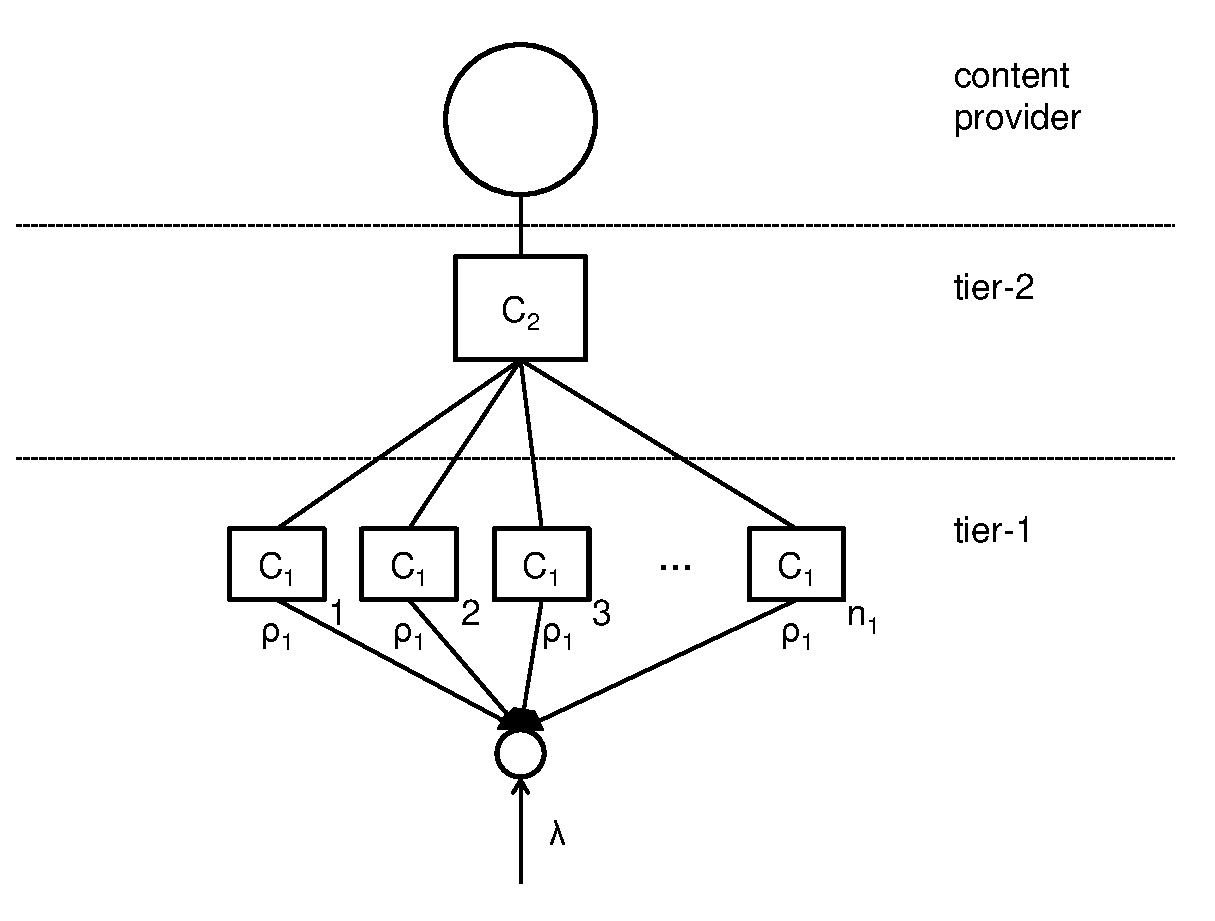
\includegraphics{cloud/figures/hcmodel}
%   \caption{Stakeholders investigated in the cloud scenarios.}
%   \label{fig:hcmodel}
% \end{figure}


The content of this chapter is published in~\cite{info3-inproceedings-2015-518,info3-inproceedings-2015-530,info3-inproceedings-2015-514,burger2016hierarchical}.
\refsec{sec:hierarchical:related_work} gives an overview on related work on the performance evaluation of caching systems and describes traffic models and analytic methods, which are relevant for the evaluation of hierarchical caching systems.
We describe the simulation model in \refsec{sec:hierarchical:simulative:simulative} and discuss the results derived to assess the potential to save inter-domain traffic in \refsec{sec:hierarchical:simulative:evaluation}.
In \refsec{sec:hierarchical:analyticbw:model} we describe our method to evaluate the performance of hierarchical systems with bandwidth constraints and give analytic results.
Numerical examples derived by analysis and simulation are given in \refsec{sec:hierarchical:analyticbw:results}.
%The simulation framework for a tiered caching architecture is described in Section~\ref{sec:simulation}.
Finally, \refsec{sec:cloud:lessons_learned} summarizes this chapter and presents the lessons learned.

\section{Background and Related Work}\label{sec:p2p:background}

This section describes background of this chapter and presents related work. We start with an overview on measurement studies of live BitTorrent networks and show different approaches to reduce inter-ISP traffic discussed in the ALTO working group of the IETF. Finally, we introduce studies that infer the inter-AS relations based on BGP routing information.
We briefly describe the structure of the YouTube video CDN and give a short introduction in the principles of crowdsourcing.
Further, we summarize related work in the field of distributed active measurements of CDNs as well as work related to crowdsourcing aided network measurements.

\subsection{Measurements and Models of Live BitTorrent Networks}

BitTorrent is a peer-to-peer file-sharing protocol, which is based on multi-source downloads between the users. All the users, i.e., \textit{peers}, sharing the same file belong to a \textit{swarm}. To join the swarm, a peer requests addresses of other peers at an index server called \textit{tracker}. In the standard BitTorrent algorithm the tracker uses random peer selection to select a subset of peers that are in the swarm. Then, the joining peer tries to establish a neighbor relation to the peers it got from the tracker and collects all peers which accepted the request in his \textit{neighbor} set. The peer signals interest to all neighbors which have parts of the file it still needs to download. To which neighbor a peer is willing to upload data is decided by the choking algorithm, which is explained in \cite{cohen:bt}.

As basis of our methodology for modeling inter-ISP BitTorrent traffic, the results in \cite{Hossfeld2011} are revisited. In \cite{Hossfeld2011} the authors provide measurements of a large number of live BitTorrent swarms taken from popular index servers such as \emph{The Pirate Bay}, \emph{Mininova}, and \emph{Demonoid}. Using the IP addresses of the peers, the authors associate every peer with its AS and estimate the potential of ALTO mechanisms based on the differentiation between local peers (peers in the same AS) and remote peers located in other ASes. In contrast, we consider the actual Internet topology in this work, i.e., the inter-ISP relations, the ISP classification in the Internet hierarchy, and the AS paths between the peers in order to estimate the optimization potential of ALTO mechanisms.

The authors of \cite{Kryczka2011} use the peer exchange protocol (PEX) in order to measure the neighbor set of all peers participating in a number of live BitTorrent swarms. Based on this information, they model the graph topology of the swarms and compare the structure to random graphs. They also investigate clustering of peers within ASes and countries, but do not focus on inter-AS relations and AS paths between peers as we do in this work.

In addition, there are measurement studies that examine and model distinct features of BitTorrent networks. In \cite{Izal2004}, a single swarm was measured for five months with a focus on the download times of the peers. Additional parameters such as the peer inter-arrival times in the swarm, their upload capacity and their online time are considered in \cite{Pouwelse2005}. The authors of \cite{Guo2005} investigate these parameters also in multi-swarm scenarios. Finally, \cite{Zhang2010} measures \unit[4.6]{million} torrents to provide an overview of the entire BitTorrent ecosystem with its different communities and index servers. Our study differs from these works in that it focuses on the location of the peers in the Internet and the AS paths between the peers.

\subsection{ALTO Mechanisms and Their Performance Evaluation}

Various mechanisms to reduce the inter-ISP traffic generated by BitTorrent and other P2P applications are currently being investigated. Besides caching of BitTorrent traffic \cite{Lehrieder2010a,Lehrieder2012,Pacifici2012}, which might involve legal issues, changing standard BitTorrent algorithms is a promising approach. The authors of \cite{Aggarwal2007} propose to use an oracle service provided by the ISP guiding the peers in their peer selection process. The evaluation uses a Gnutella network and shows that intra-AS traffic is increased significantly without a negative impact on the overlay graph. Similar approaches are proposed for BitTorrent. Bindal et al. \cite{Bindal2006} reduce the inter-ISP traffic by modifying the neighbor set of the BitTorrent peers, which can be done at the tracker or enforced by the ISPs using deep packet inspection. Their simulations use a uniform peer distribution over ASes and show a high optimization potential of this approach. The authors of \cite{Xie2008} propose to use \emph{iTrackers} to guide the peers and formulates an optimization problem to find the best neighbor sets. Finally, Oechsner et al. \cite{Oechsner2009} propose to change the choke algorithm of BitTorrent to further reduce inter-ISP traffic and evaluate it via simulations in homogeneous scenarios. The BitTorrent plugin \emph{Ono} \cite{Choffnes2008} uses the servers of content distribution networks (CDN) as landmarks and estimates the proximity of two peers by the similarity of the CDN re-direction behavior.

The authors of \cite{gkantsidis2006planet} investigate analytically the capabilities of a P2P-based content distribution network and the impact of locality. In contrast to our work, they use traffic characteristics which arise from software updates and do not consider AS relationships.
A set of evaluations of ALTO mechanisms uses scenarios inspired by measurements of live BitTorrent swarms \cite{Cuevas2011,Blond2011,Lehrieder2011}. The studied scenarios consider heterogeneous peer distributions where some ASes contain more peers of a specific swarm than others. Nevertheless, they do not take into account inter-AS relations and the AS paths between two peers. This is different in our study. Using the AS affiliation of peers and the data obtained from Caida.org, we infer the actual paths of the BitTorrent connections in the Internet. In addition, we focus on the inter-ISP relations and investigate to which degree selfish ISPs profit from recommending their peers to preferentially use connections to peers located in lower tier ASes.

\subsection{Measurements of AS Relations and Topologies}

Autonomous systems are individual parts of the Internet, which are operated by ISPs.
On a technical level, the traffic exchange between the ASes is controlled by the Border Gateway Protocol (BGP)\cite{trangia2009}. However, commercial relations between ISPs determine the routing policies configured via BGP.
%The traffic exchanged between autonomous systems is inter-domain traffic. It is differentiated from intra-domain traffic, which is the traffic in the autonomous system.
An ISP must buy transit services to access parts of the Internet it neither owns nor can access by its customers.
Hence, to route traffic between autonomous systems ISPs engage in business relationships.
These business relationships are usually not open for public but they can be abstracted into three common types \cite{gao2001}.
The relationship between two ASes can be customer-to-provider (c2p), peer-to-peer (p2p) or sibling-to-sibling (s2s).
A customer-to-provider link is present if the customer AS pays the provider AS for transit service, i.e., the provider forwards the traffic of the customer and its customers. In a peer-to-peer relation the ASes have an agreement that they exchange each others traffic and the traffic of their customers, without paying each other. Sibling-to-sibling are links between ASes of the same organization. These relations are defined in business agreements and kept secret, but they can be inferred by analyzing the routing between autonomous systems.

The approach that is most widely used to infer AS relationships is analyzing BGP routing tables. The data set used in this work is also produced by inferring BGP tables as described in \cite{dimitropoulos2007relationships}. Therefore, AS links are extracted from RouteViews BGP tables. First sibling-to-sibling links are identified by looking up organizations that own multiple AS numbers. Then customer-to-provider relationships are inferred by a heuristic that is based on the idea of relaxing the requirement for a maximal number of valid paths and using the AS degree information to detect paths that are invalid. Most challenging is the inference of peer-to-peer links since paths remain valid if peer-to-peer links are replaced by a customer-to-provider or provider-to-customer link. The authors of \cite{dimitropoulos2007relationships} develop a heuristic which combines the strengths of previous approaches by \cite{gao2001} and \cite{di2003computing}. The inferred relationships were validated by surveys, showing that \unit[96.5]{\%} customer-to-provider, \unit[82.8]{\%} peer-to-peer, and \unit[90.3]{\%} sibling-to-sibling of the inferred relationships are correct.

\subsection{Evolution and Structure of Content Delivery Networks}
%To understand why distributed measurements are necessary and to provide the basic ideas of content delivery network structures, we briefly describe the evolution of content delivery networks and the functionality of the YouTube CDN.
Since the launch of the YouTube service content delivery has drastically changed.
While the amount of traffic transported over peer-to-peer networks remained about the same, the traffic transported by content delivery networks has increased exponentially \cite{cisco2015}.
The number of users watching videos on demand has massively increased and the bandwidth to access videos is much higher.
Furthermore, the increased bandwidth enables web services to be interactive by using dynamic server- or client-side scripts.
The appearance of dynamic services and the increasing quality of multimedia content raised user expectations and the demand on the servers.
To bring content in high quality to end-users with low latency and to deal with increasing demand, content providers have to replicate and distribute the content to get it close to end-users.
Thus, content delivery networks such as the Google CDN evolved.

The global expansion of the CDNs also changes the structure of the Internet.
Google has set up a global backbone which interconnects Google's data centers to important edge points of presence.
Since these points of presence are distributed across the globe, Google can offer direct peering links to access networks with many end users.
Such, access network providers save transit costs, while Google is able to offer services with low latency.
To bring content even closer to users ISPs can deploy Google servers inside their own network to serve popular content, including YouTube videos~\cite{gcc}.

To select the closest server for a content request and to implement load balancing CDNs use the Domain Name System (DNS).
Typically a user watches a YouTube video by visiting a YouTube video URL with a web browser.
The browser then contacts the local DNS server to resolve the hostname.
Thereafter, the HTTP request is directed to a front end web server that returns an HTML page including URLs for default and fallback video servers.
These URLs are again resolved by DNS servers to physical video servers, which stream the content.
The last DNS resolution can happen repeatedly until a server with enough capacity is found to serve the request.
Thus, load balancing between the servers is achieved~\cite{adhikari2012vivisecting}.

\subsection{Crowdsourcing}
Crowdsourcing is an emerging service in the Internet that enables outsourcing jobs to a large, anonymous crowd of users~\cite{articles2013-113}.
So called \emph{Crowdsourcing platforms} act as mediator between the users submitting the tasks, the \emph{employers}, and the users willing to complete these tasks, the \emph{workers}.
All interactions between workers and employers are usually managed through these platforms and no direct communication exits, resulting in a very loose worker-employer relationship.
The complexity of Crowdsourcing tasks varies between simple transcriptions of single words~\cite{vonAhn2008} and even research and development tasks~\cite{innocentive}.
Usually, the task description are much more fine granular than in comparable forms in traditional work organization~\cite{conf2011-417}.
This small task granularity hold in particular for \emph{micro-tasks}, which can be completed within a few seconds to a few minutes.
These tasks are usually highly repetitive, e.g., adding textual descriptions to pictures, and are grouped in larger units, so called \emph{campaigns}.

\subsection{Distributed Measurements of }
There already exist a number of publications which study the structure of the YouTube CDN and its selection of video servers.
A distributed active measurement platform is necessary for these evaluation, because the CDN mechanisms consider the client locations, both geographical as well as in terms of the connected access network.
In \cite{torres2011dissecting} two university campus networks and three ISP networks were used to investigate the YouTube CDN from vantage points in three different countries.
The results show that locality in terms of latency is not the only factor for video server selection.

While the view of five different ISPs on a global CDN is still narrow, the authors of \cite{adhikari2011you} used PlanetLab  to investigate the YouTube server selection strategies and load-balancing.
They find that YouTube massively deploys caches in many different locations worldwide, placing them at the edge of the Google autonomous system or even at ISP networks.
The work is enhanced in \cite{adhikari2012vivisecting}, where they uncover a detailed architecture of the YouTube CDN, showing a 3-tier physical video server hierarchy.
Furthermore, they identify a layered logical structure in the video server namespace, allowing YouTube to leverage the existing DNS system and the HTTP protocol.

However, to assess the expansion of the whole YouTube CDN and its cache locations in access networks, the PlanetLab platform, which is located solely in NRENs, is not suitable, since it does not reflect the perspective of end users in ISP access networks.
Therefore, a different distributed measurement platform is used in \cite{rafetseder2011exploring} which runs on end user equipment and thus implies a higher diversity of nodes and reflects the perspective of end user in access networks.
However, the number of nodes that was available for the measurement is too small to obtain a global coverage of vantage points

To achieve both, the view of access networks and a high global coverage with a large number of measurement points, the participation of a large number of end users in the measurement is necessary.
Bischof et al. \cite{bischof2011crowdsourcing} implemented an approach to gather data form peer-to-peer networks to globally characterize the service quality of ISPs using volunteers.

In contrast to this we propose using a commercial crowdsourcing platform to recruit users running a specially designed measurement software and therewith act as measurement probes.
In comparison to other approaches using volunteers, this approach offers better scalability and controllability, because the number and origin of the participants can be adjusted using the recruiting mechanism of the crowdsourcing platform.
This is confirmed by Table~\ref{tab:CvsS} which compares a crowdsourcing study with a social network study quantitatively. The crowdsourcing study  is described in \cite{bookchapter2013-18}. The study is designed to assess the subjective QoE for multimedia applications, like video streaming.
The same study was conducted additionally in a social network environment for recruiting test users.
Table~\ref{tab:CvsS} shows that acquiring people in crowdsourcing platforms takes very short time compared to asking volunteers in a social network, which allows adding participants easily.
Furthermore, the completion time of the campaign of 31 hours is much shorter compared to the 26 days for the social network campaign.
Finally, in the crowdsourcing campaign workers can be selected according to their country, which allows distributing the campaign on many different countries. In the social network the coverage of countries depends on the network of user groups, which spread the campaign.
Hence, it is easy to control the number and origin of subjects participating in a crowdsourcing campaign and the completion time is considerably fast, which makes the campaign scalable and controllable. The price you pay is the reward for the workers that summed up to a total of 16 Euro for that campaign.

\begin{table}[tb]
\caption{Quantitative Comparison: Crowdsourcing / Social Network Study.} \label{tab:CvsS}
\begin{center}
{\footnotesize
	\begin{tabular}{|p{.29\textwidth}|p{.29\textwidth}|p{.29\textwidth}|} \hline
		\textbf{} & \textbf{Crowdsourcing (C)} & \textbf{Social network (S)} \\ \hline
		\textbf{Implementation time} & about 2 weeks; test implemented via dynamic web pages, application monitoring & same as for (C) \\ \hline
		\textbf{Time for acquiring people} & 5 minutes & 2 hours, as users (groups) were asked individually \\ \hline
		\textbf{Campaign submission cost} & 16 Euro & 0 Euro \\ \hline
		\textbf{Subject’s reward} & 0.15 Euro & 0 Euro \\ \hline
		\textbf{Number of test conditions} & 3 & 3 \\ \hline
		\textbf{Advertised  people} & 100 & 350 \\ \hline
		\textbf{Campaign completion time} & 31 hours & 26 days; strongly depends on advertised user groups however \\ \hline
		\textbf{Participating users} & 100 & 95 \\ \hline
		\textbf{Reliable users (very strict filtering of users)} & 30 & 58 \\ \hline
		\textbf{Number of different countries of subjects} & 30 & 3; strongly depends on users groups however \\ \hline
		\end{tabular}
}
\end{center}
\end{table}



The Internet Census Dataset was validated forensically in \cite{dainotticaida}.
In \cite{krenc2014internet} the scope of the dataset is taken into perspective and show that, although there are some qualitative problems, the measurement data seems to be authentic.
We use the Internet Census Dataset to determine the number of active IP-addresses for each autonomous system in the Internet.
%To the best of our knowledge, this is the first work which evaluates a gl
%To the best of our knowledge this is the first work which uses crowdsourcing for a distributed active measurement platform.

\section{Simulative Evaluation of Hierarchical Caching Systems}\label{sec:hierarchical:simulative:simulative}

We develop an event-based simulation framework to evaluate the performance of content delivery networks.
The results derived from the simulative evaluation are used to validate the analytic models.
The simulation framework further allows considering complex system characteristics in the performance evaluation that are not covered by the analytic models, such as the transit costs charged on inter-domain links.

%A hierarchical content delivery network with bandwidth constraints has been evaluated by simulation in \cite{applegate2010optimal}.
%The impact of using edge resources with limited capacity for content delivery on QoE is evaluated by means of simulation in \cite{info3-inproceedings-2015-530}.
In the following we describe the simulation model and investigate the benefit of overlays networks in hierarchical caching systems.
We use the model for transit traffic, c.f. \refsec{sec:p2p:methodology}, to assess the potential to save costs produced by inter-domain traffic.

\subsection{Simulation Model}\label{sec:simeval}

The parameters considered in the content delivery simulation framework are
\begin{enumerate}
  \itemsep0em
  \item the resource distribution,
  \item the caching and content placement strategy,
  \item the resource selection strategy,
  \item the content demand,
  \item the AS-Topology.
\end{enumerate}
Other considered parameters that are not relevant for this monograph, are
\begin{enumerate}
  \itemsep0em
  \item the social network of users,
  \item the video bitrate and chunk-size distribution,
  \item and the application and QoE.
\end{enumerate}
In the following we briefly describe each of the parameter sets and provide models.

\subsubsection{Resource Distribution}
The resource distribution determines how video streaming sources are distributed among autonomous systems.
The number and size of autonomous systems is specified.
The size of an autonomous system is given by the number of end-users located in it.
In literature, the distribution of end-users on ASs is characterized as heterogeneous \cite{Hossfeld2011}.
We use a geometric distribution as a basic model for number of end-users in the ASs.
A more detailed model is developed using the Internet Census dataset, c.f. \refsec{sec:aslevel:census}.
Video streaming sources can be a) data centers of the content provider, b) edge caches of the content provider, c) caches hosted by the ISP, d) home router / NaDas, or e) end-user devices.
For each video streaming source the AS-location and its capacity is specified.
The capacity is given by the number of items that can be cached.
The size of the item catalogue is also specified in this parameter set.

The cache resources can have bandwidth constraints specified by the mean and the standard deviation of the upload bandwidth.
If the upload bandwidth of a cache is limited, the service time of an object is calculated according to the available bandwidth and the object size.
The service times of the objects served by a cache are updated if the upload bandwidth changes or if an object request arrives or is completed.
Requests are blocked by a cache if the available bandwidth is below a certain threshold, or if the cache is busy serving a request.

\subsubsection{Caching and Content Placement Strategy}
The caching and content placement strategy determines in which video streaming source which video item is placed and when.
The content placement strategy is defined by the caching strategies of the individual caches.
In a distributed approach each cache decides based on the information it has, which items to cache.
Thus, the availability of items in ASs might for example be increased.
If global knowledge of the item demand is assumed, optimized content placement strategies such as hot warm cold can be used.
Each caching strategy is further defined by its specific parameters according to \refsec{sec:hierarchical:background:strategies}.

\subsubsection{Resource Selection Strategy}
The resource selection strategy determines from which cache instance an item is streamed when requested.
The simplest resource selection just selects a random resource.
In hierarchical content delivery networks, resources in tier-1 are selected first, by default.
Other resource selection strategies that try to optimize different metrics were implemented.
E.g., local resource selection tries to save inter-domain traffic by prioritizing caches in the order: home router / NaDa in the same AS, ISP managed cache in the same AS, edge cache of content provider, data center of content provider.
%Further resource selection strategies that are not yet implemented could for example consider load balancing of the request based on the capacity of the caches.

\subsubsection{Social Network of Users}
The social network of users determines the friendship relationships between users. A basic model only defines the number of users in the system.
The number of friends of the user can be modeled by a power-law or geometric distribution.
A more detailed model specifies the friendship graph which consists of a node for each user and edges between users with friend relationships.
Friendship graphs have typical properties, such as a heavy-tailed in and out degree distribution.
In literature are different models for generating graphs with these properties.
A model used to generate social network graphs with varying size and density is the forest fire model \cite{leskovec2005graphs}.
We further specify the feed size as parameter that represents the news feed of social network platforms.
The news feed is updated in sharing events.
Videos which are on the news feed of a user are watched with higher probability.
Categories are defined by specifying the probability that a user is interested in a particular category.

\subsubsection{Traffic and Popularity Model}
The content demand determines the request rates of the video items.
Different demand models are implemented in the simulation, that reach from basic models that only consider the popularity distribution of the items, to detailed models that consider temporal, spatial and social dynamics, c.f. \refsec{sec:hierarchical:background:traffic}.

The arrival process of video requests is specified by the inter-arrival time of video requests.
The request rate depends on the time of day and is generally lower at night.
The day is divided in short time slots, where the arrival rate does not change significantly, so that the arrival process can be assumed as quasi stationary.
In these time slots the arrival process is modeled as Poisson-process.
The parameter lambda of the arrival process depends on the popularity of the item and the time of day.
The probability of sharing a watched video is given by the sharing probability.

\subsubsection{Autonomous System Topology}
In order to estimate the amount of inter-domain traffic and transit costs produced, and AS topology with AS paths can be specified.
The AS paths connect the caches and data centers providing the content with the users consuming the content.
For that purpose the AS paths are inferred from AS relationships as in \refsec{sec:p2p:methodology}.
Assuming that the number of users is proportional to the number of IP addresses in an AS, we use the results of the Internet Census Dataset evaluation in \refsec{sec:aslevel:census}, to determine the distribution of users on ASs.

Finally, Simulation parameters are specified that define the random number seed, the simulation time and the parameter study.

\subsubsection{Performance metrics}

Of the total number of $n$ object requests to a cache, the objects of $k$ requests are stored in the cache and can potentially be served by the cache.
Due to bandwidth constraints some of the $k$ requests may be blocked, such that only $k'\leq k$ of the $n$ object requests are served by the cache.
To assess the performance of content delivery networks several metrics are considered:

\begin{enumerate}
\item Cache hit rate $p_\text{hit}$: The ratio of requests to a cache that find the object in the cache (cache hit) to the total number of requests to the cache
\begin{equation}
  p_\text{hit}=\frac{k}{n} \, .
\end{equation}
\item Cache serve rate $p_\text{serve}$: The ratio of requests to a cache that find the object in the cache and that are not blocked due to bandwidth constraints to the total number of requests to the cache
\begin{equation}
  p_\text{serve}=\frac{k'}{n} \, .
\end{equation}
\item Cache contribution: The share of all requests that is served by a cache.
\item Inter-domain traffic: The share of requests by users in an AS that cannot be served by a cache in the same AS.
\end{enumerate}

\begin{figure}[bt]
  \centering
  \includegraphics[width=0.8\textwidth]{hierarchical/simulative/figures/watch}
  \caption{Proccess diagram of a WATCH event.}
  \label{fig:WATCH}
\end{figure}

The content delivery simulation framework is implemented in MatLab.
The simulation is event-based including two major events.
First, the WATCH event, which is processed when a user watches or consumes a video item.
Second, the SHARE event, which simulates a sharing action of a user, where the video is posted on the news feeds in the social network.
\reffig{fig:WATCH} shows the process diagram of a WATCH event.
The process of a WATCH event starts by selecting a video according to the specified demand model.
A video identifier $v_\text{id}$ is returned.
In the next step a cache or data center is selected according to the resource selection strategy that holds the item with $v_\text{id}$.
The download of the item from the selected resource is recorded in the statistics.
The cache identifier $c_\text{id}$ is returned and the cached items are updated according to the caching strategy specified in the parameters.
The user then decides to share $v_\text{id}$ with probability $p_\text{share}$.
In this case a SHARE event is queued.
Finally, the next WATCH event is queued according to the traffic and popularity model.

A SHARE event puts a given $v_\text{id}$, or a random video according to the user's interest on top of the news feed of the user's friends.
The user's friends are determined by the social graph.
The simulation is initialized with a WATCH event for each user.

The simulation framework is open source and available on github\footnote{\url{https://github.com/pettitor/content_delivery}}.

\subsection{Numerical Examples and Impact on Transit Costs}\label{sec:hierarchical:simulative:evaluation}

To evaluate the performance of a CDN supported by home routers, two scenarios are simulated. The first scenario simulates requests to a CDN with caches organized in a tree structure and compares isolated caches to cooperating caches to assess the benefit of the overlay.
The second scenario adds an AS topology with peering and transit links to evaluate the inter-domain traffic saving potential.
As described in \refchap{chap:aslevel}, a transit link exists between a customer ISP and its transit provider, if the customer ISP pays the transit provider to forward its traffic destined to parts of the Internet that the customer ISP does not own or cannot reach.

%\subsection{Caching}
% To assess the impact of the number of shared home routers and the size of the ISP, a tiered caching architecture with resource locations at three different tiers, including the main data center of the content provider, CDN caches, and end-user equipment is evaluated.
% The number of different content items to be downloaded or streamed from the resources is specified by the catalog size $N$. Tier-3 resource is the data center of the content provider, where all $N$ content items are stored. Tier-2 resources are edge caches and ISP caches, typically organized in a CDN, which are located close to Internet exchange points or within ISP networks. Requests served by ISPs or edge caches produce less or no inter-domain costs. Thus, these caches are referred as ISP caches in the following. The capacity of ISP caches is given as a fraction of $N$ and is specified by $C_\text{ISP}$. The caching strategy of ISP caches is LRU.
%Each autonomous system hosts an ISP cache.
Within tier-1, the caches are placed on shared home routers. These caches are referred to in the following as home routers (HRs). The cache capacity of HRs is specified by $C_1$ and their caching strategy is LRU. In this study $C_1$ is set to four (4) content items.
We evaluate the performance dependent on the autonomous system size $n_\text{user}$, in terms of the number of end-users in the autonomous system. The probability that an end-user enables the HR to shares contents is given by $p_\text{share}$. The probability that a user requests certain content items depends on the content's popularity distribution, which is specified by the Zipf exponent $\alpha$.

\subsubsection{Benefits of an Overlay}

To evaluate the performance of the overlay, two cases are considered (a) the tree case and (b) the overlay case. In the tree case (a), each user is assigned to one shared HR in its AS. If a user shares its HR, it is assigned only to its HR. A requested item is looked up in the assigned HR initially, i.e. in the tier-3 cache. If the requested item is not found, the request is forwarded to the next tier. The hierarchical caching strategy is leave-copy-everywhere, which means that the video is cached in each cache on the look up path. In the overlay case (b), a requested item is looked up in the HR of the user, if it is not found, it is looked up in shared HRs in the same autonomous system using the overlay. If no tier-3 cache in the AS contains the item it is looked up in tier-2 caches and finally in the data center of the content provider. The hierarchical caching strategy is leave-copy-everywhere, too, with the constraint, that the item is cached in the tier-3 cache only, which was looked up first.

\begin{figure}[tb]
  \centering
  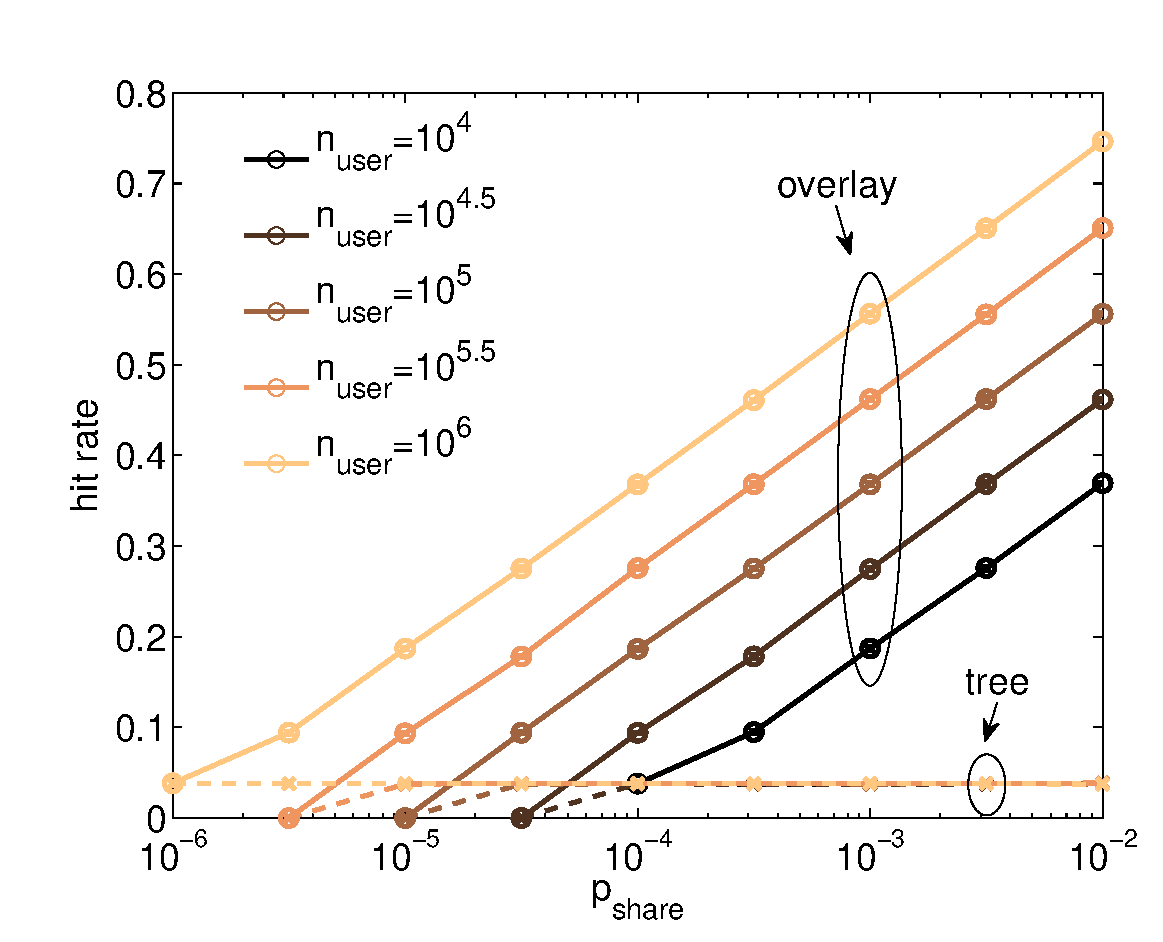
\includegraphics[width=0.7\textwidth]{hierarchical/simulative/figures/overlay_nuser_hitrate3}
  \caption{Hit rate of the overlay dependent on home router sharing probability.}
  \label{fig:overlay_nuser_hitrate}
\end{figure}

\begin{figure}[tb]
  \centering
  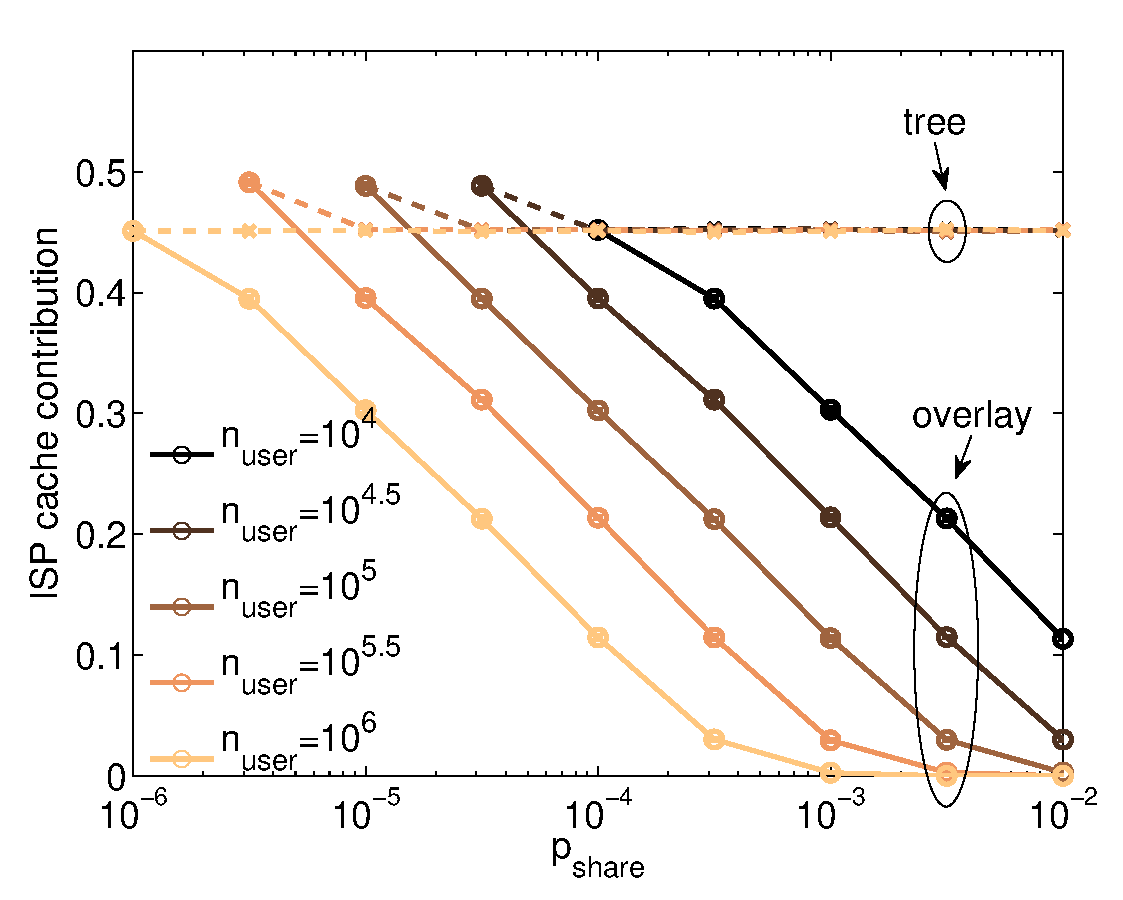
\includegraphics[width=0.7\textwidth]{hierarchical/simulative/figures/overlay_nuser_ISPcontrib3}
  \caption{ISP cache contribution dependent on home router sharing probability.}
  \label{fig:overlay_nuser_ISPcontrib}
\end{figure}

\begin{figure}[tb]
  \centering
  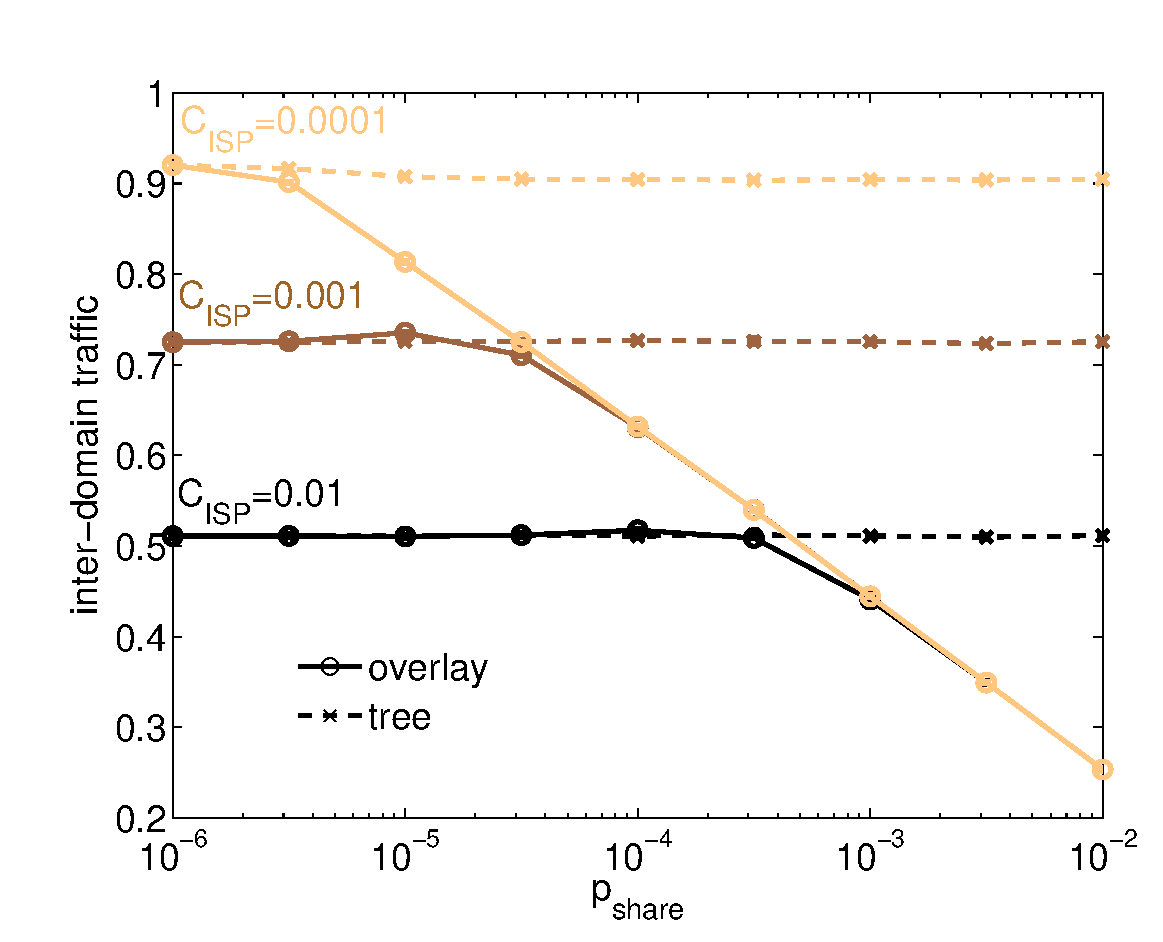
\includegraphics[width=0.7\textwidth]{hierarchical/simulative/figures/overlay_interdomain3}
  \caption{Inter-domain traffic dependent on home router sharing probability.}
  \label{fig:overlay_interdomain}
\end{figure}

% \begin{figure*}[tb]
% \centering
% \begin{subfigure}[t]{0.49\textwidth}
% 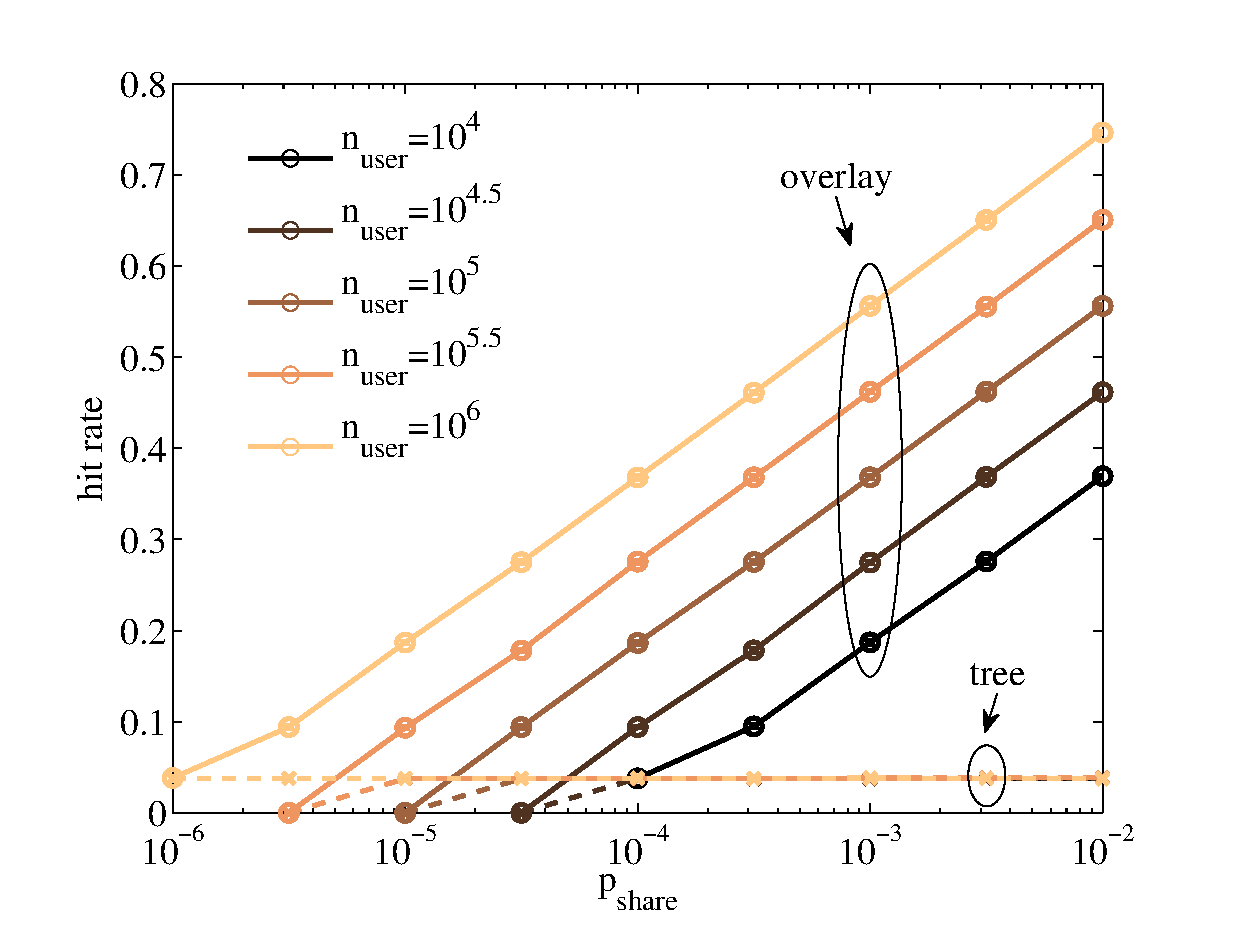
\includegraphics[width=\textwidth]{hierarchical/simulative/figures/overlay_nuser_hitrate}
% \caption{Hit rate of the overlay}
% \label{fig:overlay_nuser_hitrate}
% \end{subfigure}
% \begin{subfigure}[t]{0.49\textwidth}
% 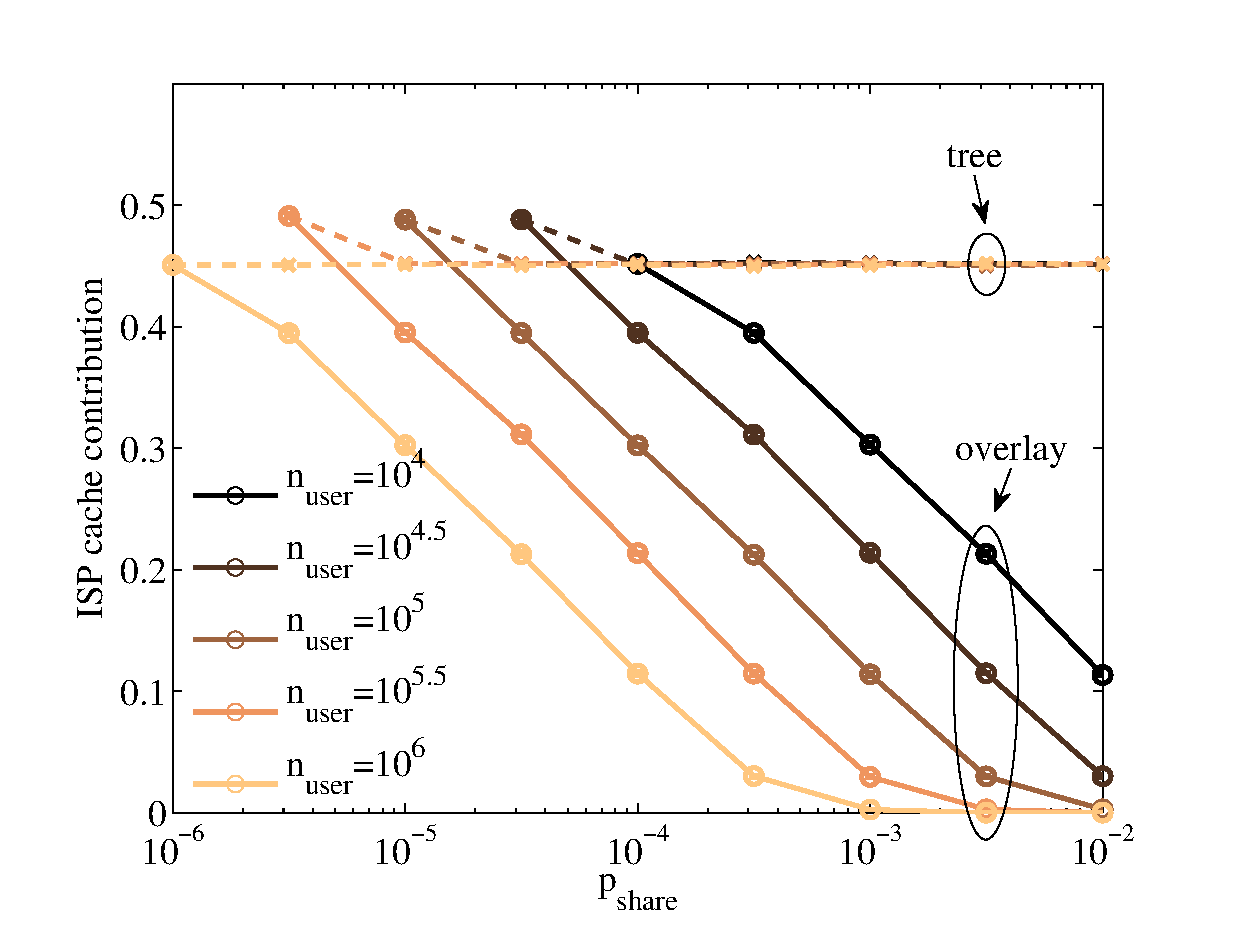
\includegraphics[width=\textwidth]{hierarchical/simulative/figures/overlay_nuser_ISPcontrib}
% \caption{ISP cache contribution}
% \label{fig:overlay_nuser_ISPcontrib}
% \end{subfigure}
% \begin{subfigure}[t]{0.49\textwidth}
% 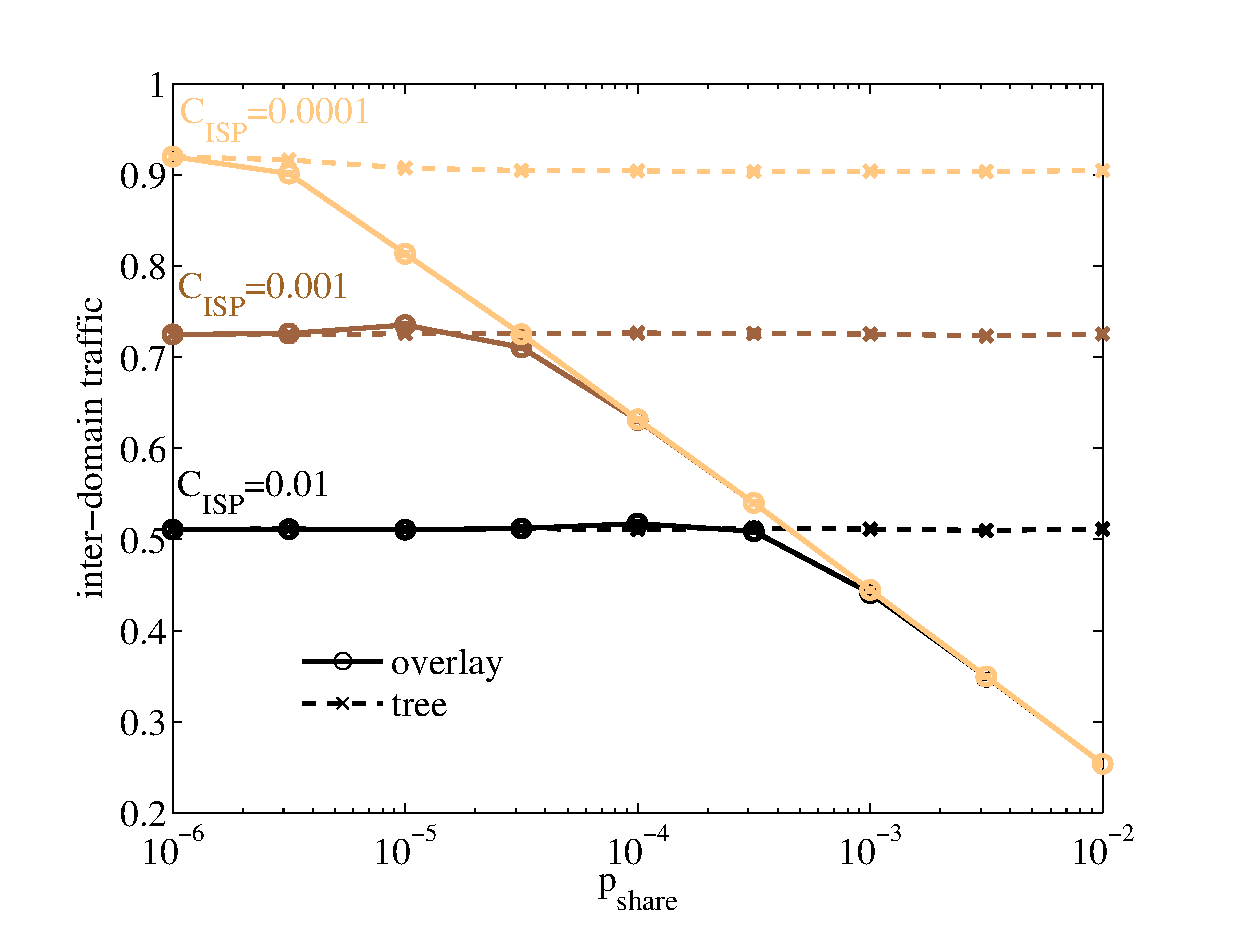
\includegraphics[width=\textwidth]{hierarchical/simulative/figures/overlay_interdomain}
% \caption{Inter-domain traffic}
% \label{fig:overlay_interdomain}
% \end{subfigure}
% \caption{Overlay and ISP cache contribution and inter-domain traffic dependent on home router sharing probability.}
% \end{figure*}

As the goal of this evaluation is to assess the potential of the overlay and to identify success scenarios, the simulation model assumes that the upload rate of caches is unlimited. However, in practice the upload rate limits the number of requests that can be served by a cache, especially for smaller devices like HRs. The evaluation uses a static and global popularity distribution. In practice the item request process is dynamic and dependent on personal and regional preferences.
The simulation uses a catalog size of $N=10^6$. The results obtained show the average of ten simulation runs with $10^6$ requests and their respective 95\% confidence intervals.
%The hierarchic caching strategy is leave-copy-down, which means that the video is cached in a certain tier only if it is already available in a higher tier.
%In the following we evaluate the performance of the tiered caching architecture. By studying the impact of the home router sharing probability, we identify the amount of home routers, which needs to be shared so that such a mechanism pays off for ISPs. We vary the ISP cache capacity and the Zipf exponent \alpha to investigate to what extent the load on ISP caches can be reduced and how the system performs under various request patterns. For each configuration 5 simulation runs were conducted to achieve significance. The results show the mean value of the 5 runs with 95\% confidence intervals.

Figure~\ref{fig:overlay_nuser_hitrate} shows the hit rate of the overlay dependent on the sharing probability for a constant ISP cache capacity of $C_\text{ISP}=0.01$. In the tree case, where each user is assigned to a HR as a tier-3 cache, the hit rate is independent of the sharing probability. The hit rate is limited by the cache capacity of the HR. If HRs are organized in an overlay, their hit rate increases with the sharing probability, since requested content items are looked up in all HRs belonging to the overlay. This shows that an overlay highly increases the performance of a caching system with a high number of small caches. Hence, the overlay highly benefits providers and end-users. The hit rate increases with the size of AS $n_\text{user}$, as a higher total cache capacity is available.

%\begin{figure}[tb]
%\centering
%\includegraphics[width=75mm]{overlay_ISPhitrate}
%\caption{ISP cache hit rate dependent on sharing probability.}
%\label{fig:overlay_ISPhitrate}
%\end{figure}

%Figure~\ref{fig:overlay_ISPhitrate} shows the ISP cache hit rate dependent on the home router sharing probability. The ISP cache hit rate decreases in the overlay case, since popular items are served by the overlay. The ISP cache is only requested for unpopular items which are less likely to be hit. Without overlay the ISP cache gets more efficient with increasing sharing probability, since the branching factor of the tree increases.

%\begin{figure}[tb]
%\centering
%\includegraphics[width=75mm]{overlay_ISPcontrib}
%\caption{ISP cache contribution dependent on sharing probability.}
%\label{fig:overlay_ISPcontrib}
%\end{figure}

Figure~\ref{fig:overlay_nuser_ISPcontrib} shows the ISP cache contribution dependent on the sharing probability for a constant ISP cache capacity of $C_\text{ISP}=0.01$. In a tree structure the sharing probability has no significant impact on the ISP cache contribution. This depends on the fact that the hit rate of tier-3 caches is low and independent of the sharing probability. All remaining requests are forwarded to the ISP cache and in case of a hit the ISP cache contributes. If the HRs are organized in an overlay, the ISP cache contribution decreases because more requests can be served from the overlay. In this case the ISP cache also gets less efficient because it is only requested for rare items that are not cached in the overlay.
For large ASs with a high number of end-users the ISP cache contribution approaches zero, if at least every thousandth user shares its HR. In this case the ISP cache can be shut down, which saves operating costs and energy. This shows that especially large ASs can benefit from an overlay.

%\begin{figure}[tb]
%\centering
%\includegraphics[width=75mm]{overlay_local}
%\caption{Share of requests served locally dependent on sharing probability.}
%\label{fig:overlay_ISPcontrib}
%\end{figure}

Figure~\ref{fig:overlay_interdomain} shows the inter-domain traffic dependent on the sharing probability for an AS with $n_\text{user}=10^6$ end-users. If no overlay is present the sharing probability has close to no impact on the amount of requests served locally. In this case the inter-domain traffic can only be reduced by increasing the ISP cache capacity. In the overlay case the number of requests served locally increases with the sharing probability, which decreases the inter-domain traffic. Dependent on the ISP cache capacity a higher fraction of shared HRs is necessary to reduce inter-domain traffic.

\subsubsection{Inter-Domain Traffic}

The overlay is not only used to access content from HRs in the same AS, but also from HRs in neighboring ASs. If the neighboring AS is a peering or customer ISP, no transit costs are incurred.
To assess the inter-domain traffic saved, an AS topology is added to the simulation. The AS relationship dataset provided by caida.org\cite{caida2015} of January 2015 is used and it specifies peering and customer-to-provider links of each AS. The data set consists of 46,172 ASs and 177,000 links.
To be able to process the simulation the topology is limited to RIPE NCC EU ASs. The remaining subset still consists of 31,256 ASs and 77,382 links.
The number of users per AS is determined by evaluating the Internet Census Dataset\cite{carna2013}, which provides a scan on active IP addresses in the Internet. Assuming that the number of users in an AS is proportional to the number of active IP addresses and the probability of a user being in an AS is set accordingly.
To save costly inter-domain traffic and to mitigate load on ISP caches, the following resource selection policy is applied:

If an item is not found on enabled HRs in the same AS, it is requested from other resources in the order:
%(1) HRs in peering ISP ASs, (2) HRs in customer ISP ASs, (3) ISP cache in local AS, (4) ISP cache in peering ISP ASs, (5) ISP cache in customer ISP ASs, and (6) content provider.
%\vspace{2mm}
\begin{enumerate}
	\itemsep0em
	\item HRs in peering ISP ASs
	\item HRs in customer ISP ASs
	\item ISP cache in local AS
	\item ISP cache in peering ISP ASs
	\item ISP cache in customer ISP ASs
	\item content provider
\end{enumerate}

\begin{figure}[tb]
  \centering
  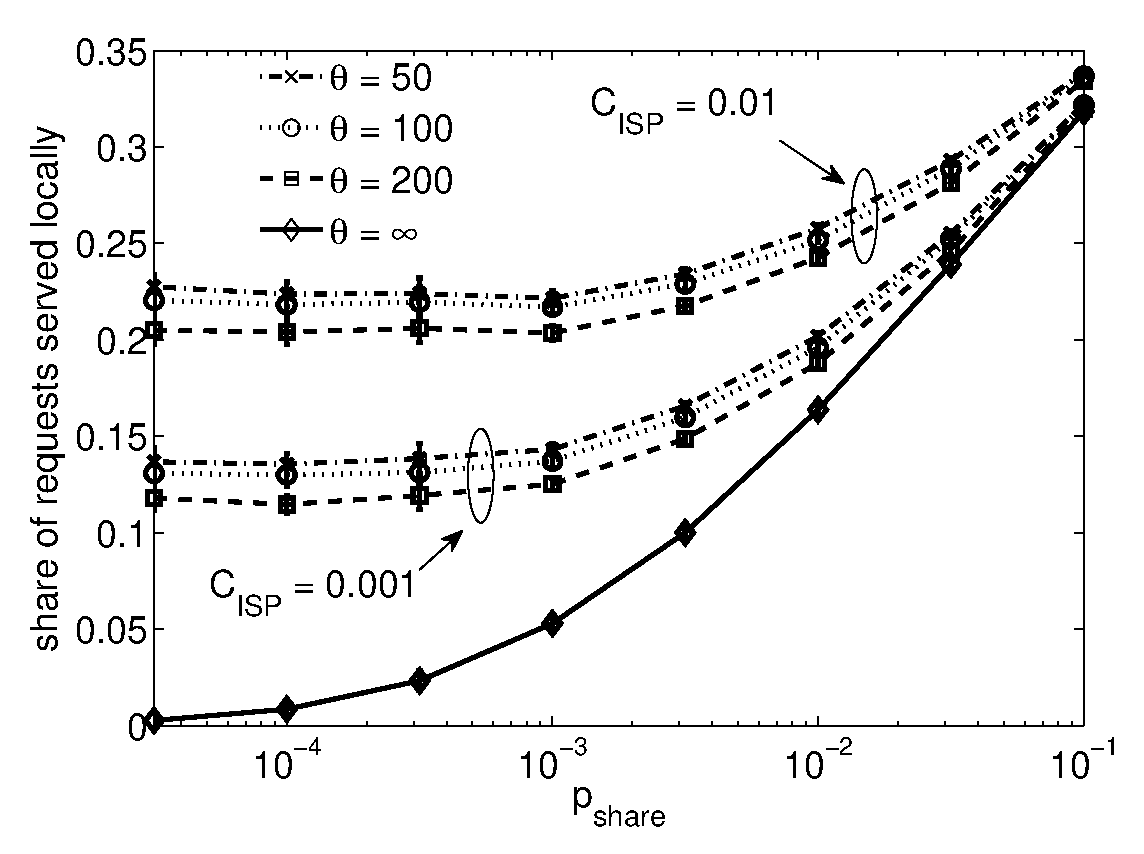
\includegraphics[width=0.7\textwidth]{hierarchical/simulative/figures/RBHlocal3}
  \caption{Share of requests served locally dependent on sharing probability.}
  \label{fig:RBHlocal}
\end{figure}

\begin{figure}[tb]
  \centering
  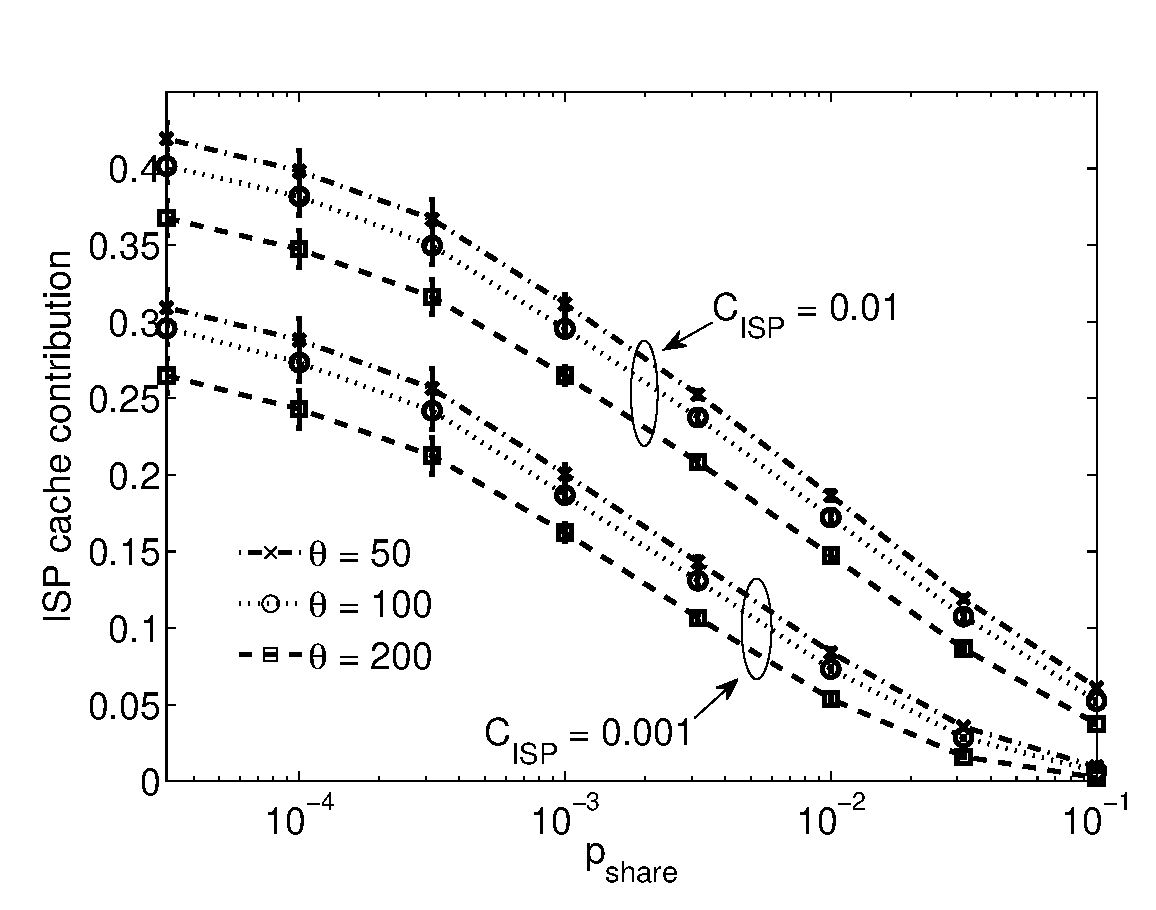
\includegraphics[width=0.7\textwidth]{hierarchical/simulative/figures/ISPcontrib3}
  \caption{ISP cache contribution dependent on sharing probability.}
  \label{fig:ISPcontrib}
\end{figure}

\begin{figure}[tb]
  \centering
  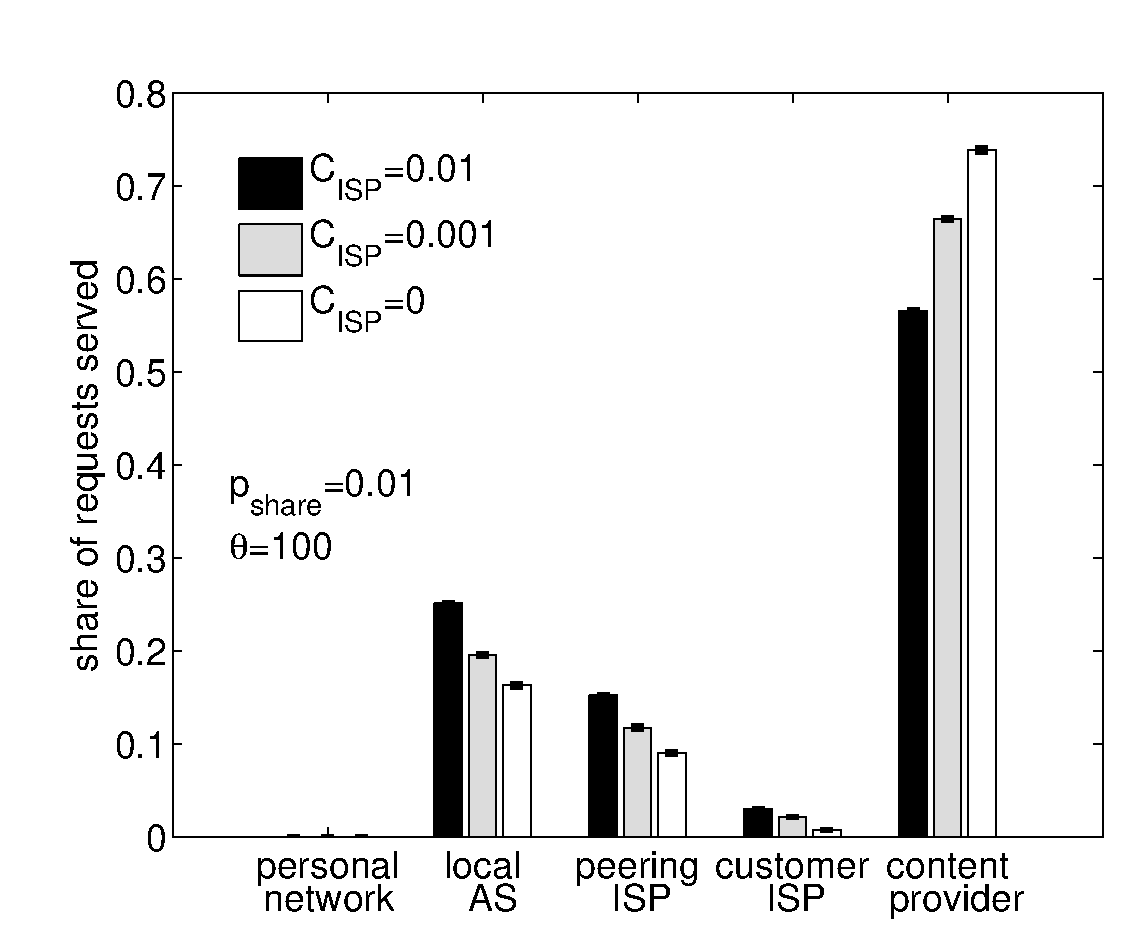
\includegraphics[width=0.7\textwidth]{hierarchical/simulative/figures/RBHall3}
  \caption{Share of requests served per domain.}
  \label{fig:RBHall}
\end{figure}

% \begin{figure*}[ht]
% \centering
% \begin{subfigure}[t]{0.49\textwidth}
% \includegraphics[width=\textwidth]{hierarchical/simulative/figures/RBHlocal}
% \caption{Share of requests served locally}
% \label{fig:RBHlocal}
% \end{subfigure}
% \begin{subfigure}[t]{0.49\textwidth}
% 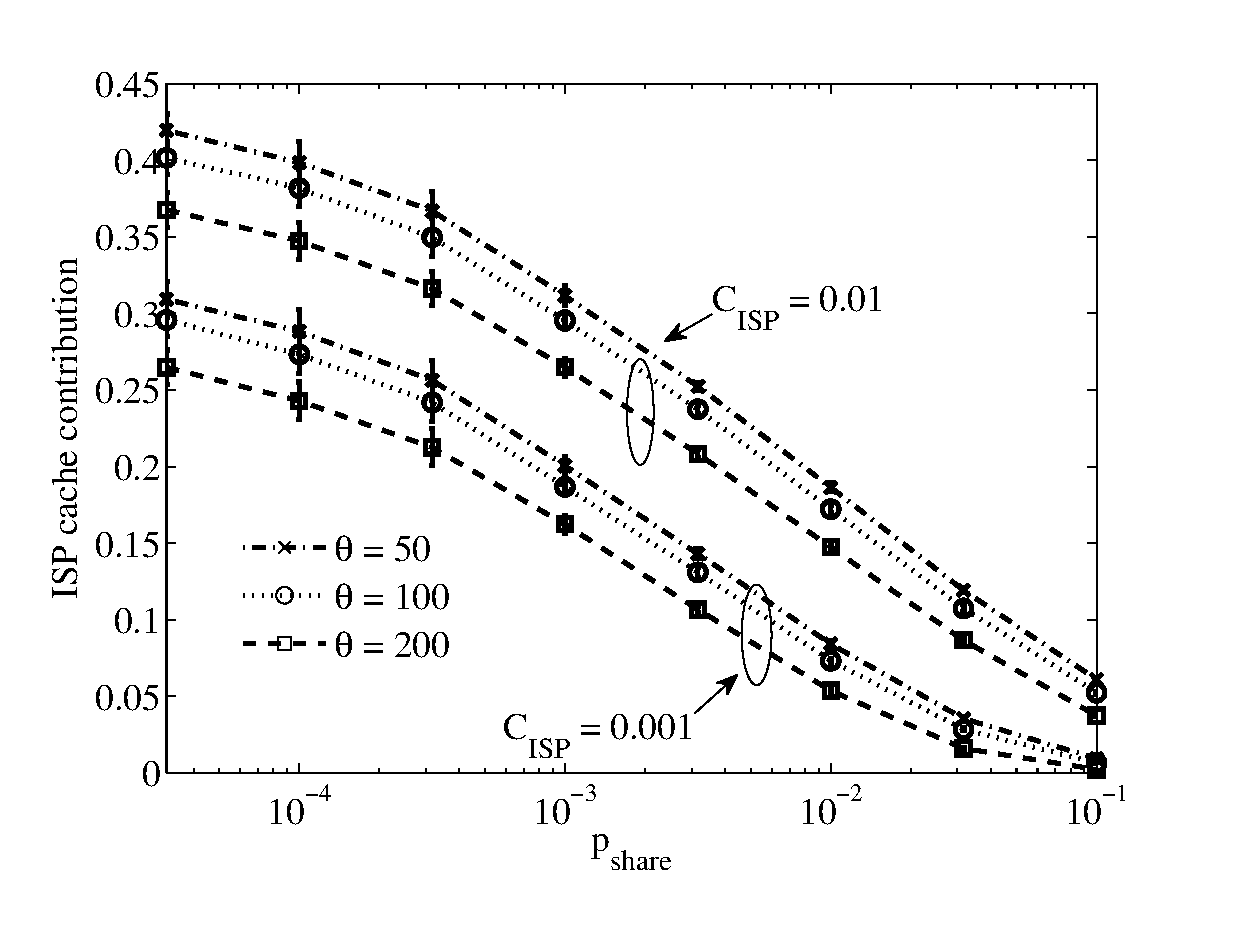
\includegraphics[width=\textwidth]{hierarchical/simulative/figures/ISPcontrib}
% \caption{ISP cache contribution}
% \label{fig:ISPcontrib}
% \end{subfigure}
% \begin{subfigure}[t]{0.49\textwidth}
% \includegraphics[width=\textwidth]{hierarchical/simulative/figures/RBHall}
% \caption{Share of requests served per domain}
% \label{fig:RBHall}
% \end{subfigure}
% \caption{Share of requests served locally and ISP cache contribution dependent on sharing probability and share of requests served per domain.}
% \end{figure*}

A policy designed to prioritize ISP caches to remote HRs did not have a significant impact on traffic savings.
%The capacity of ISP caches $C_\text{ISP}=\{0.001,0.01\}$ is relative to the catalogue size.
The threshold $\theta$ specifies the minimum number of users an AS must have to host an ISP cache. If $\theta=\infty$ no AS hosts an ISP cache and content delivery is solely supported by HRs.
To investigate the performance of our approach, the impact of the HR sharing probability $p_\text{share}$ on the inter-domain traffic and on the ISP cache contribution is studied. The share of traffic within the local AS, peering and customer-to-provider links is evaluated.
For the generation of content item requests a Zipf popularity distribution with slope $\alpha=0.99$ was applied.

%\begin{figure}[tb]
%\centering
%\includegraphics[width=75mm]{RBHlocal}
%\caption{Share of requests served locally dependent on sharing probability.}
%\label{fig:RBHlocal}
%\end{figure}

Figure~\ref{fig:RBHlocal} shows the share of requests served locally dependent on the HR sharing probability. More than 20\% of requests can be served locally, if the ISP cache can store 1\% of the catalog size. With an increasing threshold $\theta$ the number of ASs hosting an ISP cache decreases and, thus, the share of requests being served locally. If the number of shared HRs increases, more traffic can be kept locally. This effect is stronger for a lower ISP cache capacity. In case of $\theta=\infty$ where no ISP caches are available, the sharing probability has the strongest impact on inter-domain traffic. For a high sharing probability the ISP cache size has only little impact on the inter-domain traffic.

Figure~\ref{fig:ISPcontrib} shows the ISP cache contribution dependent on the HR sharing probability. The number of requests an ISP cache can serve increases with its capacity. As for the inter-domain traffic, the sharing probability has a high impact on the ISP cache contribution. For high sharing probabilities the ISP cache contribution approaches zero. This means that ISP caches can be shut down, if a sufficient amount of users would share their HRs.
For a lower threshold $\theta$ more ISP caches are deployed and the ISP cache contribution increases.

%\begin{figure}[tb]
%\centering
%\includegraphics[width=75mm]{RBHall}
%\caption{Share of requests served per domain.}
%\label{fig:RBHall}
%\end{figure}

To study the requests served per domain, the HR sharing probability is set to 1\% and the threshold $\theta$ to 100 users.
Figure \ref{fig:RBHall} shows the share of requests served per domain. Almost none of these requests can be served by the personal HR. This might depend on the fact that items are requested according to a global popularity distribution.
If personal interests are considered in the demand model, higher hit rates and contributions from personal caches are expected. Dependent on the ISP cache capacity, 20 to 25\% of requests can be served locally and 15 to 20\% from neighboring ASs. Still about 2 out of 3 requests are served by the content provider. This depends on the fact that with Zipf slope of $\alpha = 0.99$ content item requests are highly heterogeneous. In practice, temporal and social dynamics of users' interests will lead to temporal and local correlations in requests, which improve the performance of local and personal caches.

%\input{hierarchical/analytic/analytic}
\section{Analysis of Caching Systems with Bandwidth Constraints}\label{sec:hierarchical:analyticbw:model}

To evaluate content delivery networks based on the number of available home routers and their limited capacity, we define a system model for a tiered caching architecture.
Tier-1 caches are on leaf nodes such as home routers, caches of the content delivery network are in tier-2 and ultimately tier-3 is the content provider.
We use analytic models to calculate the efficiency of the tiered caching architecture.



%\subsection{Performance Metrics}

%\begin{itemize}
%	\item hit rate, define as hit on device WITH enough available bandwidth / resources
%	\item effective cache capacity
%  \item ...
%\end{itemize}

%To be able to estimate the costs for ASes arising from transit services, we need to know how much traffic is generated and how much providers charge customers for forwarding the traffic.
%We consider a snapshot and assume instantaneous traffic rates, i.e., the file-size of the download can be neglected.
%For simplicity we make assumptions on how much traffic is generated in each swarm, depending on the the number and location of peers.
%\newtheorem{A}{Assumption}\begin{A}\label{npeers}
%The traffic generated by a peer is equally shared among its neighbors.
%\end{A}
%\newtheorem{B}[A]{Assumption}\begin{B}\label{ntraffic}
%All peers generate traffic at the same rate.
%\end{B}
%\newtheorem{C}[A]{Assumption}\begin{C}\label{npaths}
%The traffic between ASes is equally shared among the paths that connect them.
%\end{C}
%In practice traffic rates are allocated by BitTorrent's choking algorithm and traffic is generally not shared among different AS paths. But, since we consider the aggregated traffic of a large number of swarms, we argue that these assumptions are reasonable and that the results are not changed significantly.

\subsection{Analytic Performance Models for Caching Systems}

In the following we provide analytic models to evaluate the performance of a tiered caching architecture.
We use existing models for systems without bandwidth constraints in order to determine baselines and upper bounds for comparison.
We then show our approach to determine the hit rate of hierarchical cache networks with bandwidth constraints.

\subsubsection{The Che-approximation}

We first consider the Che-approximation \cite{che2002hierarchical} for the simple case of a single cache with LRU policy.
Let $C$ be the capacity of the single cache.
$T_C(m)$ is the cache eviction time of object $m$, i.e., the time needed before $C$ objects, not including $m$, are requested at the cache.
Object $m$ is in the cache if the last request for object $m$ is less than $T_C$ in the past.
For Poisson arrivals, the probability that an object $m$ is in the cache equals the probability that the inter-request time for object $m$ is smaller than $T_C$.
Let $A_m$ be a random variable for the inter-arrival time for requests of object $m$.
The probability that $A_m$ is smaller than $T_C$ is given by the cumulative distribution function, which is exponentially distributed:

\begin{equation}
	p_\text{hit}(m) = p_\text{in}(m) = P(A_m \leq T_C) = 1-e^{-\lambda_m T_C} \, .
\end{equation}

Due to the memoryless property of the Poisson process the hit probability equals the stationary probability that an item $m$ is in the cache.

We define the indicator function $\chi_m$ to determine if item $m$ is in the cache.

\begin{equation}
\chi_m =
	\begin{cases}
		1, & m \, \text{in cache} \, ,\\
      		0, & \text{otherwise} \, .
	\end{cases}
\end{equation}

Following \cite{martina2014unified}, we obtain for the cache capacity $C$:

\begin{equation}
	C=\sum_m{\chi_m} \, ,
\end{equation}

and

\begin{equation}
	C=\mathbb{E}\left[\sum_m{\chi_m}\right]=\sum_m{\mathbb{E}\left[\chi_m\right]}=\sum_m{p_\text{in}(m)} \, .
\end{equation}

after averaging both sides.

$T_C$ is the only unknown in the above equation and can be determined by a fixed point iteration.
Thus, the interaction among the contents is summarized by the cache eviction time $T_C$, which allows decoupling the dynamics of the different contents.

The overall hit probability is calculated by considering the probability $p_m$ of requesting item $m$

\begin{equation}
p_\text{hit}=\sum_m p_m p_\text{hit}(m) \, .
\end{equation}

\subsubsection{No bandwidth constraints}

We use the Che-approximation for the LRU cache hit rate to calculate the baseline given by the cache hit rate of the tier-2 cache without tier-1 cache support $p'_\text{hit}(2)$. The characteristic time $T_{C_2}$ depends on the capacity of the tier-2 cache $C_2$ and is determined by a fixed point approximation

\begin{equation}
p_\text{hit}(2,m)=p_\text{in}(2,m)=1-e^{-\lambda_{m}T_{C_2}} \, .
\end{equation}

The overall hit probability in tier-2 is calculated by considering the probability $p_m$ of requesting item $m$

\begin{equation}
p'_\text{hit}(2)=\sum_m p_m p_\text{hit}(2,m) \, .
\end{equation}
%\begin{equation}
%p_m=\frac{\lambda_m}{\sum_i \lambda_i}
%\end{equation}

To calculate the maximum hit rate for LRU, we assume that tier-1 caches are completely organized with the tier-2 cache, and the capacity of tier-1 caches is added to the tier-2 cache capacity

\begin{equation}
\hat p_\text{hit}(m)=\hat p_\text{in}(m)=1-e^{-\lambda_{m}T_{(C_2+n_1\cdot C_{1})}} \, .
\end{equation}

It is practically not feasible to control the capacity of all tier-1 caches and coordinate them with the tier-2 cache.
To still bundle the capacity of the tier-2 caches, the caches can form an overlay.

%The probability to find object $m$ in a tier-2 cache is $p_{in}(2,m)$.

%TODO tree case.

%\begin{equation}
%p_\text{hit}(2,m)=p_{in}(2,m)=1-e^{-\lambda_{m}T_{C_2}}
%\end{equation}

If an overlay is used, the requests that cannot be served by the personal tier-1 cache are forwarded to other tier-1 caches in the overlay, before they are forwarded to the tier-2 cache.
%The requests that are forwarded to the tier-1 cache have looked up the object $m$ in all tier-2 caches.
%The requests for object $m$ forwarded to tier-1 $\lambda_m^o(1)$ are not hit by any of the $n_2\approx p_{share}\cdot n_{user}$ tier-2 caches.

We approximate the hit rate of the overlay by calculating the hit rate of a tandem network with two caches according to \cite{martina2014unified}. The tandem network consists of the tier-2 cache and a cache that has the sum of capacities of tier-1 caches. The miss stream of the consolidated tier-1 cache is forwarded to the tier-2 cache.
The replacement strategy in the network is leave-copy-down, that means that an item is only placed in a cache if it is found in a higher tier cache. Thus only frequently requested items are propagated to lower tier-caches, which makes them more efficient. The Che-approximation can be applied to tandem networks by determining $p_\text{in}(1,m)$ for the tier-1 caches

\begin{equation}
p_\text{in}(1,m) = 1-e^{\lambda(1,m)T_{n_1 C_1}} \, .
\end{equation}

The hit probability is no longer equal to the probability that an item is in the cache, as the cache miss stream arriving at the tier-2 cache is no longer Markov. According to \cite{martina2014unified} the hit probability can then be determined by:

\begin{multline}
p_\text{hit}(1,m) = ((1-p_\text{in}(1,m))p_\text{hit}(2,m) + p_\text{in}(1,m)) \\ \cdot(1-e^{\lambda(1,m)T_{n_1 C_1}}) \, .
\end{multline}

The rate of the miss stream $\lambda(2,m)$ arriving at the tier-2 cache can then be determined as

\begin{equation}
\lambda(2,m) = (1-p_\text{in}(1,m))\lambda(1,m) \, .
\end{equation}

The probability that an item is in the tier-2 cache is approximated assuming exponentially distributed inter request times

\begin{equation}
p_\text{hit}(2,m) = p_\text{in}(2,m) = 1-e^{\lambda(2,m)T_{C_2}} \, .
\end{equation}

The total hit rate in tier-$i$ is then calculated by considering the probability of an item $m$ being requested at tier-$i$ cache $p(i,m)$

\begin{equation}
p_\text{hit}(i) = \sum_{m}p(i,m)p_\text{hit}(i,m), i\in\{1,2\} \, .
\end{equation}
%if tC(2) > tC(1)
%   phit(2,:) = (1-exp(-l(2,:).*(tC(2)-tC(1))))+(1-phit(2,:)).*(1-exp(-l(1,:)*tC(1)));
%else
%   phit(2,:) = (1-phit(2,:)).*(1-exp(-l(1,:)*tC(2)));
%end

% wrong
%\begin{equation}
%\lambda_m^o(1)=\lambda_m\cdot(1-p_\text{hit}(2,m))^{n_2}
%\end{equation}

%The hit rate of the object $m$ in tier-1 cache in the overlay case $p_\text{hit}^{o}(1,m)$ can be approximated according to \cite{•}.

%\begin{equation}
%p_\text{hit}^{o}(1,m) \approx 1-e^{A_1^o(m)}
%\end{equation}

%where (TODO improve)
%\begin{align*}
%A_1^o(m)&=\frac 1 {n_2}\cdot \lambda_m\cdot (1-p_{in}(2,m))^{n_2}\cdot max(0,T_{C_1}-T_{C_2}) + \\ &\frac {n_2-1}{n_2}\cdot \lambda_m\cdot(1-p_{in}(2,m))^{n_2}\cdot T_{C_1}
%\end{align*}

%The hit rate of the tier-2 overlay caches $p_\text{hit}^{o}(2,m)$ is the probability of the event complementary to no tier-2 cache hit.

%\begin{equation}
%p_\text{hit}^{o}(2,m) = \lambda_m\cdot (1-(1-p_{in}(2,m))^{n_2})
%\end{equation}

The overall hit rate of the hierarchical caching system is then calculated by

\begin{equation}
\bar{p}_\text{hit} = p_\text{hit}(1)+(1-p_\text{hit}(1))p_\text{hit}(2) \, .
\end{equation}

%with $p_m=\frac{\lambda_m}{\sum_i \lambda_i}$.

\subsection{Analytic Model with Bandwidth Constraints}

The above hit rates only apply if tier-1 and tier-2 caches have unlimited bandwidth, which is practically not feasible.
Considering the home router scenario, the bandwidth of tier-1 caches is limited depending on the subscription and the availability of DSL.
We use the throughput of the tier-1 caches $\rho_1$ as parameter to specify the upload bandwidth available on home routers.

%\begin{equation}
%\bar b = \frac 1 N \sum_{m=1}^N b_m
%\end{equation}

%\begin{equation}
%\bar \rho_1 = \frac 1 {n_1} \sum_{i=1}^{n_1} \rho_1(i)
%\end{equation}

%\begin{equation}
%\bar\mu = \frac{\bar b}{\bar \rho_2}
%\end{equation}

The offered traffic of item $m$ at tier-1 cache $k$ can be calculated by the quotient of the arrival rate per cache $\frac{\lambda_m}{n_1}$ and the mean service rate, which is determined by the bitrate $b_m$ and the duration $d_m$ and the link throughput $\rho_1$ in case of video contents

\begin{equation}
a(m,k) = \frac{\lambda_m \cdot b_m \cdot d_m}{n_1\cdot \rho_1(k)} \, .
\end{equation}

The total offered traffic of item $m$ is $a(m) = \sum_k a(m,k)$.

%\begin{equation}
%a(m) = \sum_k a(m,k) \, .
%\end{equation}

The content placement in tier-1 is specified by $X: N \times n_1\mapsto \{0,1\}, X(m,k) = 1$, if content $m$ is placed at cache $k$, else $0$.

According to \cite{valancius2009greening} an optimal placement of items in terms of minimum loss rate in the stationary case is achieved by the hot-warm-cold content placement.
Hot content with $a(m)\geq n_1$ is placed on each cache.
Warm content is placed on $\lfloor a(m) \rfloor$ caches.
Cold content is not placed on any of the caches.
The constraint  $\forall k, \sum_m X(m,k)\leq C_1(k)$ has to be met, such that the cache capacities are not exceeded.
%hotwarmcold: while $\forall k, \sum_m X(m,k)\leq C_1(k)$
%\begin{itemize}
%	\item $\forall k, X(m,k)=1, \text{if}\ a(m) \geq \sum_k C_1(k) $
%	\item $\forall i, X(m,k)=1, i$ not occ TODO
%\end{itemize}

% We define the indicator function $\chi_m$ to determine if item $m$ is cached.
%
% \begin{equation}
% \chi_m =
% 	\begin{cases}
% 		1, & \exists k : X(m,k)=1 \\
%       		0, & \text{otherwise}
% 	\end{cases}
% \end{equation}

%The hit rate of the placement can be calculated by
%%TODO correct?
%\begin{equation}
%	p_\text{hit}^\text{hwc}(2,m) = \chi_m \cdot (1-\max(0,\frac{a(m)}{n_2}-1))
%\end{equation}

%and

%\begin{equation}
%	p_\text{hit}^\text{hwc}(2) = p_\text{hit}^\text{hwc}(2,m) \cdot p_m \, .
%\end{equation}

%TODO leave out
% The effective cache size of tier-1 $C_1^*$ is defined as the number of different items that is stored in tier-1 caches. It is calculated by
%
% \begin{equation}
% C_1^* = \sum_m \chi_m \, .
% \end{equation}

Since not every hit can be served by tier-1 caches because of their limited bandwidth, we consider the loss rate $p_{b}(1,m)$, which is defined as the share of requests of item $m$ that is not hit in tier-1 or is blocked if none of the tier-1 caches storing the requested item has enough bandwidth left to serve the request.

Let $\nu_m$ be the number of tier-1 caches that hold item $m$

\begin{equation}
\nu_m=\sum_{k=1}^{n_1} X(m,k) \, .
\end{equation}

%An item is not hit, if it is not placed in any of the tier-1, hence, if $X(m,k)=0 \forall k\in {1,\ldots,n_1}$.
An item is not hit, if it is not placed in any tier-1 cache, i.e., if $\nu_m=0$.
If an item is placed in at least one of the tier-1 caches, i.e., $\nu_m>0$, we approximate the blocking probability by the Erlang formula for a loss system with $\nu_m$ servers with mean service rate $\mu_{m} = \frac{\rho_1}{b_m\cdot d_m}$ and arrival rate $C_1\lambda_m$:


\begin{equation}
p_{b}(1,m) =
	\begin{cases}
		\frac{\frac{a_m^{\nu_m}}{m!}}{\sum_{k=0}^{\nu_m}\frac{a_m^k}{k!}}, & \nu_m>0 \\
    1, & \text{otherwise} \, ,
	\end{cases}
\end{equation}

where we approximate the offer of item $m$ with
\begin{equation}
a_m \approx \frac{\lambda_m\cdot C_1}{\mu_m} \, .
\end{equation}
Note, that here we assume that the arrival rate of requests of the $C_1$ items stored in the cache is equal to the rate of item $m$.
In order to calculate the exact stationary distribution of the blocking probability, the arrival rate of requests has to be conditioned on the feasibility of the content placement, which is too complex to evaluate.
Refer to \cite{tan2013optimal} for details.
%We also tried other arrival rates, such as average arrival rate of the items cached, which did not improve the approximation.

The blocked requests are forwarded to the tier-2 cache and the arrival rate of requests of item $m$ at the tier-2 cache can be determined as

\begin{equation}
	\lambda_m(2) = \lambda_m\cdot p_\text{b}(1,m) \, .
\end{equation}

We determine the hit rate of the tier-2 cache $p_\text{hit}(2)$ again by using the Che-approximation for cache capacity $C_2$ and arrival rates $\lambda_m(2)$, assuming that the miss stream of the tier-1 caches follows a Poisson process

%TODO describe
\begin{equation}
	p_b(1) = \sum_m p_m p_{b}(1,m) \, .
\end{equation}

The total rate of requests hit and served by tier-1 and tier-2 caches is then determined by

\begin{equation}
	p_\text{hit} = (1-p_b(1)) + p_b(1)\cdot p_\text{hit}(2) \, .
\end{equation}

In order to assess the benefit of the tiered architecture compared to a single ISP cache, we define the cache hit rate gain $\omega$ as the normalized difference of the total hit rate $p_\text{hit}$ and the cache hit rate of the tier-2 cache $p'_\text{hit}(2)$ without tier-1 cache support

\begin{equation}
\omega = \frac{p_\text{hit}-p'_\text{hit}(2)}{p'_\text{hit}(2)} \, .
\end{equation}

%\begin{equation}
%X_{m,k} =
%	\begin{cases}
%		0, & \text{if}\ a()=1 \\
%      		1, & \text{otherwise}
%	\end{cases}
%\end{equation}
%\begin{equation}
%r\leq C_2 n_{user} p_{share}
%\end{equation}
%\begin{equation}
%X\leq C_2 n_{user} p_{share}
%\end{equation}

%effective capacity of hot warm cold overlay -> che approximation two tiered LCD.
%Metric efficiency gain hit rate / hitrateLRU(C1)

\subsection{Measurement Results}
\label{sec:results}

In this section we show the results of the distributed measurement of the global CDN.
The obtained results show the distribution of clients and servers over different countries.
Furthermore, the mapping on autonomous systems gives insights to the coverage of the Internet.

\subsubsection{Distribution of Vantage Points on Countries}

To investigate the coverage of measurement points we study the distribution of the PlanetLab nodes and Crowdsourcing workers.
Figure~\ref{fig:PLSrc} shows the distribution of PlanetLab nodes on countries over the world.
The pie chart is denoted with the country codes and the percentage of PlanetLab nodes in the respective country.
Most of the 220 clients are located in the US with 15\% of all clients.
However, more than 50\% of the clients are located in West-Europe.
Only few clients are located in different parts of the world.
The tailored distribution towards Western countries is caused by the fact, that the majority of the PlanetLab nodes are located in the US or in western Europe.

\begin{figure}[bt]
    \centering
	\begin{subfigure}[t]{0.49\textwidth}
	\includegraphics[width=\textwidth]{aslevel/crowd/results/figs/PLSrc.pdf}
\caption{PlanetLab}
\label{fig:PLSrc}
\end{subfigure}
\begin{subfigure}[t]{0.49\textwidth}
	\includegraphics[width=\textwidth]{aslevel/crowd/results/figs/MWSrc.pdf}
\caption{Crowdsourcing}
 	\label{fig:MWSrc}
\end{subfigure}
    \caption{Distribution of measurement points on countries in a) PlanetLab and b) Crowdsourcing platform.}
    \label{fig:Src}
\end{figure}

%\begin{figure}[tb]
%	\centering
% 	\includegraphics[width=0.5\textwidth]{figures/Diagramme/Geo/PLSrc.pdf}
%  	\caption{Distribution of PlanetLab nodes over countries.}
%  	\label{fig:PLSrc}
%\end{figure}

Figure~\ref{fig:MWSrc} shows the geo-location of workers on the crowdsourcing platform.
In contrast to PlanetLab, most of the 247 measurement points are located in Asia-Pacific and East-Europe.
The majority of the participating workers 20\% are from Bangladesh followed by Romania and the US with 10\%.
This bias is caused by the overall worker distribution on the platform~\cite{conf2011-410}. However, this can be influences to a certain extend by limiting the access to the tasks to certain geographical regions.
%The payment for crowdsourcing tasks is equal for all countries.
%Hence, the reward is higher for people living in developing countries with less value of money.
%This makes crowdsourcing platforms interesting for people in these countries and leads to a tailored distribution of clients towards different parts of the world.

%\begin{figure}[tb]
%	\centering
% 	\includegraphics[width=0.5\textwidth]{figures/Diagramme/Geo/MWSrc.pdf}
%  	\caption{Distribution of microworkers over countries.}
%  	\label{fig:MWSrc}
%\end{figure}
\subsubsection{Distribution of Identified YouTube Servers on Countries}

To investigate the expansion of the YouTube CDN we study the distribution of YouTube servers over the world.
Figure~\ref{fig:PLDst} shows the location of the servers identified by the PlanetLab nodes.
The requests are mainly directed to servers in the US. Only 20\% of the requests were directed to servers not located in the US.

\begin{figure}[bt]
    \centering
	\begin{subfigure}[t]{0.49\textwidth}
	\includegraphics[width=\textwidth]{aslevel/crowd/results/figs/PLDest.pdf}
  \caption{PlanetLab}
	\label{fig:PLDst}
  \end{subfigure}
	\begin{subfigure}[t]{0.49\textwidth}
	\includegraphics[width=\textwidth]{aslevel/crowd/results/figs/MWDest.pdf}
  \caption{Crowdsourcing}
 	\label{fig:MWDst}
  \end{subfigure}
    \caption{Distribution of physical YouTube servers on countries accessed from a) PlanetLab nodes and b) workers of a crowdsourcing platform.}
    \label{fig:Dst}
\end{figure}

%\begin{figure}[tb]
%	\centering
% 	\includegraphics[width=0.5\textwidth]{figures/Diagramme/Geo/PLDest.pdf}
%  	\caption{Distribution of YouTube servers accessed from PlanetLab nodes.}
%  	\label{fig:PLDst}
%\end{figure}

The servers identified by the crowdsourcing measurement are shown in Figure~\ref{fig:MWDst}.
The amount of requests being directed to servers located in the US is still high.
44\% of clients were directed to the US.
However, in this case the amount of requests resolved to servers outside the US is higher.
In contrast to the PlanetLab measurement many requests are served  locally in the countries of clients.
Furthermore, the decrease of 80\% to 44\% of request being directed to the US shows a huge difference.

%\begin{figure}[tb]
%	\centering
% 	\includegraphics[width=0.5\textwidth]{figures/Diagramme/Geo/MWDest.pdf}
%  	\caption{Distribution of YouTube servers accessed from crowdsourcing users.}
%  	\label{fig:MWDst}
%\end{figure}

Hence, network probes being overrepresented in the US and Europe leads to a limited  view of the content delivery network and the Internet.
This shows the impact of different locations of measurement points on the view of the CDN.
It also demands a careful choice of vantage points for a proper design of experiments in distributed network measurements.
Although both sets of measurement points are globally distributed the fraction of the CDN which is discovered by the probes has very different characteristics.

The amount of servers which is located in the US almost doubles for the PlanetLab measurement.
While 44\% of the requests are resolved to US servers in the Crowdsourcing measurement, nearly all requests of PlanetLab nodes are served by YouTube servers located in the US.
Although less than 15\% of clients are in US, requests are frequently directed to servers in the US. That means that there is still potential to further distribute the content in the CDN.

\subsubsection{Coverage of Autonomous Systems with YouTube Servers}

To identify the distribution of clients on ISPs  and to investigate the expansion of CDNs on autonomous systems we map the measurement points to the corresponding autonomous systems.

%\begin{figure}[tb]
%	\centering
% 	\includegraphics[width=0.5\textwidth]{figures/valli_AS_pl_src.pdf}
%  	\caption{Distribution of PlanetLab nodes over autonomous systems.}
%  	\label{fig:AS_mw_src}
%\end{figure}
%
%\begin{figure}[tb]
%	\centering
% 	\includegraphics[width=0.5\textwidth]{figures/valli_AS_mw_src.pdf}
%  	\caption{Distribution of crowdsourcing clients over autonomous systems.}
%  	\label{fig:AS_mw_src}
%\end{figure}

Figure~\ref{fig:AS_pl_dst} shows the autonomous systems of YouTube servers accessed by PlanetLab nodes.
The autonomous systems were ranked by the number of YouTube servers located in the AS.
The empirical probability $P(k)$ that a server belongs to AS with rank $k$ is depicted against the AS rank.
The number of autonomous systems hosting YouTube servers that are accessed by PlanetLab nodes is limited to less than 30.
The top three ranked ASs are AS15169, AS36040 and AS43515.
AS15169 is the Google autonomous system which includes the Google backbone.
The Google backbone is a global network that reaches to worldwide points of presence to offer peering agreements at peering points.
AS36040 is the YouTube network connecting the main datacenter in Mountain-View which is also managed by Google.
AS43515 belongs to the YouTube site in Europe which is administrated in Ireland.
Hence, two thirds of the servers are located in an autonomous systems which is managed by Google.
Only few requests are served from datacenters not being located in a Google AS.
The reason that request from PlanetLab are most frequently served by ASs owned by Google might be a good interconnection of the NRENs to the Google ASs.

\begin{figure}[bt]
    \centering
	\begin{subfigure}[t]{0.49\textwidth}
	\includegraphics[width=\textwidth]{aslevel/crowd/results/figs/valli_AS_pl_dst.pdf}
  \caption{PlanetLab}
	\label{fig:AS_pl_dst}
  \end{subfigure}
	\begin{subfigure}[t]{0.49\textwidth}
	\includegraphics[width=\textwidth]{aslevel/crowd/results/figs/valli_AS_mw_dst.pdf}
  \caption{Crowdsourcing}
 	\label{fig:AS_mw_dst}
  \end{subfigure}
    \caption{Distribution of YouTube servers on autonomous systems from a) PlanetLab and b) Crowdsourcing perspective.}
    \label{fig:AS_dst}
\end{figure}

%\begin{figure}[tb]
%	\centering
% 	\includegraphics[width=0.5\textwidth]{figures/valli_AS_pl_dst.pdf}
%  	\caption{Distribution of YouTube servers over autonomous systems from PlanetLab perspective.}
%  	\label{fig:AS_pl_src}
%\end{figure}

Figure~\ref{fig:AS_mw_dst} depicts the autonomous systems where requests to YouTube videos from  the crowdsourcing workers were directed.
The empirical probability that a server belongs to an AS has been plotted dependent on the AS rank.
The YouTube servers identified by the crowdsourcing probes are located in more than 60 autonomous systems.
Hence, the YouTube CDN is expanded on a higher range of ASs from the crowdsourcing perspective compared to PlanetLab.
Again the three autonomous systems serving most requests are the ASs managed by Google, respectively YouTube.
But the total number of requests served by a Google managed AS is only 41\%.
Hence, in contrary to the PlanetLab measurement, requests are served most frequently from ASs not owned by Google.
Here, caches at local ISPs  managed by YouTube could be used to bring the content close to users without providing own infrastructure.
This would also explain the large number of identified ASs providing a YouTube server.
The results show that the PlanetLab platform is not capable to measure the structure of a global CDN, since large parts of the CDN are not accessed by clients in NRENs.
%The aim of this work was to compare the measurement capabilities of the concurring platforms, opposed to a complete measurement of the YouTube CDN.
%It is part of future work to perform an exhaustive measurement study based on PlanetLab and crowdsourcing platforms, which produces a representative view from gobally distributed vantage points on the YouTube CDN and its distribution on autonomous systems.

%Crowdsourcing identifies a higher range of different ASs

%\begin{figure}[tb]
%	\centering
% 	\includegraphics[width=0.5\textwidth]{figures/valli_AS_mw_dst.pdf}
%  	\caption{Distribution of YouTube servers over autonomous systems from crowdsourcing end-user perspective.}
%  	\label{fig:AS_mw_src}
%\end{figure}

%TODO identify overlaps.

%A substantial number of servers is not located in a Google AS
%Heterogeneous distribution. Implication on measurement. Optimize measurement framework?

% \input{hierarchical/social/social}
\section{Lessons Learned}\label{sec:aslevel:lessons_learned}
In this chapter we characterize content delivery networks on autonomous systems level. %by evaluating measurements of the most common content delivery principles P2P and CDN.
For that purpose we summarize related work and use measurements conducted on the distributed platform PlanetLab and a crowdsourcing platform.
To assess the potential of content delivery approaches that use local resources, e.g., on home routers, we determine the number of active IP-addresses from the Internet Census dataset.

%P2P -> CDN
%to accurately model content delivery networks ... is described.
%While ... we find three major outcomes.
First, we provide a comprehensive overview on content delivery network concepts and their evolution. We briefly describe the structure of the YouTube CDN and describe the concept of the next generation of hierarchical CDNs, which use local resources to support content delivery.
In order assess the number of local resources available in each AS, we analyze the Internet Census Dataset to derive the distribution of IP-addresses on ASs.
To this end, we use a mapping of IP-addresses to autonomous system numbers.
we find that the distribution of IP-addresses is highly heterogeneous showing that 30\% of the active IPs belong to the 10 largest autonomous systems.
This means that the potential of approaches that use resources on home routers highly depend on the ISP network.

Second, we propose the usage of crowdsourcing platforms for distributed network measurements to increase the coverage of vantage points.
We evaluate the capability to discover global networks by comparing the coverage of video server detected, using a crowdsourcing platform as opposed to using the PlanetLab platform.
To this end, we use exemplary measurements of the global video CDN YouTube, conducted in both the PlanetLab platform as well as the crowdsourcing platform Microworkers.
Our results show that the vantage points of the concurring measurement platforms have very different characteristics.
We show that the distribution of vantage points has high impact on the capability of measuring a global content distribution network.
The capability of PlanetLab to measure a global CDNs is rather low, since 80\% of requests are directed to the United States.
Our results confirm that the coverage of vantage points is increased by crowdsourcing.
Using the crowdsourcing platform we obtain a diverse set of vantage points that reveals more than twice as many autonomous systems deploying video servers than the widely used PlanetLab platform.
%Part of future work is to determine if the coverage of vantage points can be even further increased by targeting workers from specific locations to get representative measurement points for all parts of the world.

Finally, we investigate where in the Internet BitTorrent traffic is located and which ISPs benefit from its optimization. To this end, we use measurements of live BitTorrent swarms to derive the location of BitTorrent peers and data provided by Caida.org in order to calculate the actual AS path between any two peers.
Our results show that the traffic optimization potential depends heavily on the type of ISP. Different ISPs will pursue different strategies to increase revenues.
Our results confirm that selecting peers based on their locality has a high potential to shorten AS paths between peers and to optimize the overlay network. In the observed BitTorrent swarms twice as much traffic can be kept intra-AS using locality peer selection. Thus, the inter-AS traffic is almost reduced by \unit[50]{\%} in \tier and in large ISPs.
%If ...
%This would for example allow ..

Based on the results obtained in this chapter, we develop models that describe the characteristics of CDNs and the number of active subscribers in ISP networks.
The models allow us to analyze the performance of traffic management mechanisms in realistic scenarios.
%Upper bounds / potential of p2p cdn approach.
%Including the application providers as stakeholders and considering their key performance indicators requires new models but also allows us to better understand the impact of mechanisms implemented in applications.
%Key performance indicators of application providers sometimes overlap with those relevant to users, as application providers try to improve the experience of users in order to reduce churn.

%Highlighted by both, the P2P approach and the CDN approach the distribution of peers on autonomous systems and the popularity of content is highly heterogeneous.
%Dynamics (orange paper)
%While general traffic management mechanisms intent to optimize the cdn
%this only increases the efficiency of the ISP cache, which may cause suboptimal results if the popularity of videos large variance.
%Thus, we suggest to  tradeoffs, within reason, to the user.
%This approach could be seen as extending the \emph{Economic Traffic Management} approach to the user.

